%% This is file `elsarticle-template-5-harv.tex',
%%
%% Copyright 2009 Elsevier Ltd
%%
%% This file is part of the 'Elsarticle Bundle'.
%% ---------------------------------------------
%%
%% It may be distributed under the conditions of the LaTeX Project Public
%% License, either version 1.2 of this license or (at your option) any
%% later version.  The latest version of this license is in
%%    http://www.latex-project.org/lppl.txt
%% and version 1.2 or later is part of all distributions of LaTeX
%% version 1999/12/01 or later.
%%
%% The list of all files belonging to the 'Elsarticle Bundle' is
%% given in the file `manifest.txt'.
%%
%% Template article for Elsevier's document class `elsarticle'
%% with harvard style bibliographic references
%%
%% $Id: elsarticle-template-5-harv.tex 159 2009-10-08 06:08:33Z rishi $
%% $URL: http://lenova.river-valley.com/svn/elsbst/trunk/elsarticle-template-5-harv.tex $
%%

% This is for Sublime-text with LaTeXTools to compile the nomenclature table
\immediate\write18{makeindex -s nomencl.ist -o "\jobname.nls" "\jobname.nlo"}

\documentclass[preprint,authoryear,12pt]{elsarticle}

\usepackage{amssymb}
\usepackage{amsmath}
\usepackage{color}
\usepackage{soul}  % Remove on submission
\usepackage{siunitx}
\usepackage{array}
\usepackage{lineno}
\usepackage[utf8]{inputenc}
\newcommand{\rpm}{\raisebox{.2ex}{$\scriptstyle\pm$}}

\usepackage{framed} % Framing content
\usepackage{multicol} % Multiple columns environment
\usepackage{nomencl} % Nomenclature package
\makenomenclature
\setlength{\nomitemsep}{-\parskip} % Baseline skip between items

\inputencoding{utf8}

\newcommand{\code}{\texttt}

\journal{Biosystems Engineering}

\begin{document}
\begin{frontmatter}

\title{A Heavy-Duty Platform for Autonomous Navigation in Kiwifruit Orchards}

\author[UoW]{Mark H. Jones\corref{mjemail}}
\cortext[mjemail]{markhedleyjones@gmail.com}

\author[UoA]{Jamie Bell\corref{jbemail}}
\cortext[jbemail]{jamie977@gmail.com}
\author[UoW]{Daniel Dredge}
\author[UoW]{Matthew Seabright}
\author[RPL]{Alistair Scarfe}
\author[UoW]{Mike Duke}
\author[UoA]{Bruce MacDonald}

\address[UoW]{School of Engineering, University of Waikato, Hamilton, New Zealand}
\address[UoA]{Faculty of Engineering, University of Auckland, Auckland, New Zealand}
\address[RPL]{Robotics Plus Ltd, Newnham Innovation Park, Tauranga, New Zealand}

\begin{abstract}
    Horticultural robots designed for in-field use generally require a means of transport around farms or orchards.
    A common approach is to directly integrate a drive system at the expense of increasing overall complexity.
    Alternatively, robots can be modularised and attached to general purpose platforms.
    General purpose platforms reported previously are designed to carry relatively light payloads orientated toward ground based crops.
    This paper presents a modularised platform capable of carrying modules of up to \SI{1000}{\kilo\gram} beneath \SI{1.4}{\meter} high pergola-style kiwifruit canopies.
    The electrical and software architecture is discussed as well as vehicle's mechanical design.
    Sensors suitable for autonomous navigation are evaluated in-orchard and tested with prototype navigation algorithms.
    It is found that global navigation satellite system (GNSS) based navigation is not feasible under kiwifruit canopies, but perception based navigation sees the platform complete a number of block traversals autonomously.


\end{abstract}

\begin{keyword}
    Agricultural automation \sep autonomous navigation \sep sensor selection
\end{keyword}

\end{frontmatter}

\linenumbers

\begin{table*}
  \small
   \begin{framed}
     \printnomenclature
   \end{framed}
\end{table*}

\nomenclature{$\alpha$}{Slope angle (deg)}
\nomenclature{$\Delta~v$}{Change in velocity (\SI{}{\meter\per\second})}
\nomenclature{$\omega$}{Angular velocity (\SI{}{\radian\per\second})}
\nomenclature{$\tau$}{Torque (\SI{}{\newton\meter})}
\nomenclature{$B$}{Nominal width of a tyre (\SI{}{\meter})}
\nomenclature{$C_{rr}$}{Rolling resistance coefficient (unitless)}
\nomenclature{$E$}{Offset between a tyre and its axis of rotation (\SI{}{\meter})}
\nomenclature{$F_{accel}$}{Force required to accelerate (\SI{}{\newton})}
\nomenclature{$F_{grade}$}{Force due to a gradient (\SI{}{\newton})}
\nomenclature{$F_{rolling}$}{Force due to rolling resistance (\SI{}{\newton})}
\nomenclature{$F_{total}$}{Total force (\SI{}{\newton})}
\nomenclature{$G$}{Acceleration due to gravity (\SI{}{\meter\per\second\squared})}
\nomenclature{$m$}{Mass (\SI{}{\kilo\gram})}
\nomenclature{$P$}{Power (\SI{}{\watt})}
\nomenclature{$r$}{Radius of a wheel (\SI{}{\meter})}
\nomenclature{$u$}{Friction coefficient (unitless)}
\nomenclature{$v$}{Velocity (\SI{}{\meter\per\second})}
\nomenclature{$W$}{Force transmitted through a wheel (\SI{}{\newton})}
\nomenclature{CAN}{Controller Area Network}
\nomenclature{GLONASS}{A GNSS service operated by the Russian Federation}
\nomenclature{GNSS}{Global Navigation Satellite System}
\nomenclature{GPS}{An GNSS service operated by the United States}
\nomenclature{IMU}{Inertial Measurement Unit}
\nomenclature{PSA}{Pseudomonas syringae pv. actinidiae (type of bacteria)}
\nomenclature{ROS}{Robot Operating System}
\nomenclature{RTK-GPS}{Realtime Kinematic GPS}
\nomenclature{SLAM}{Simultaneous Localisation And Mapping}


\section{Introduction}
\label{sect:intro}
    Short-term labour requirements within New Zealand's kiwifruit industry peak twice a year corresponding with the pollination and harvesting of kiwifruit.
    The majority of employment during these peaks is filled by seasonal or casual workers \citep{Timmins2009}.
    As kiwifruit is the country's largest horticultural export by value \citep{StatisticsNewZealand2015}, effective automation in this industry will promote economic growth.
    Development of an automated kiwifruit harvester with integrated drive system has previously been published \citep{Scarfe2012}.
    That work presented a platform designed to autonomously navigate though pergola-style kiwifruit orchards and had four integrated harvesting arms.
    Work presented here focuses on creating a platform that operates independently from orchard related tasks, such as fruit harvesting and pollination.
    Utilisation of a generalised base platform is increased by using it during harvesting \emph{and} pollination seasons.
    Details of modules developed for use on the vehicle are published separately.
    The modules have been built as part of a larger project focusing on automation in kiwifruit orchards.

    Automated kiwifruit harvesting and pollination demands computer control, state-of-the-art manipulators, and machine-vision systems.
    These systems are bulky and have specific geometric requirements dictated by kiwifruit growing systems.
    They share the need for electrical power, air pressure, and a means of locomotion.
    However, they differ in the way they move when operating.
    The pollinating module moves at a well-known speed with minimum changes in angle.
    % This differs from the harvesting module, which advances a set distance between stationary harvesting cycles.
    This differs from the harvesting module, which advances a set distance between periods of being stationary.
    To enable the whole system to work autonomously, the platform must be able to self-drive in a way appropriate for both modules.

    While publishing details of BoniRob, a general purpose robotics platform for field use, the authors stated that ``since the robot development already includes a high complexity, the application itself should be of comparably low complexity'' \citep{Ruckelshausen2009}.
    By separating the development of the platform from other task-specific modules, the risk of a single part becoming overly complex is reduced.

    The development of autonomous vehicles in agriculture is not new, but much of the literature relates to manned vehicles converted to drive-by-wire.
    Because the canopy of a pergola-style kiwifruit orchard can droop as low as \SI{1.4}{\meter} to the ground under fruit loading, most standard vehicles are not suited to this environment.
    Many autonomous vehicles designed for use in orchards, such as vineyards, rely on Global Navigation Satellite Systems (GNSS) for guidance.
    The dense foliage of a kiwifruit canopy and the surrounding shelter-belts make receiving GNSS signals unreliable at best.
    The presented vehicle must navigate through kiwifruit orchards whilst relying only on perception-based sensors.
    Additional requirements are to:
    \begin{enumerate}
        \item support a mass of \SI{1000}{\kilo\gram},
        \item have a maximum height of \SI{1.4}{\meter},
        \item provide \SI{8}{\kilo\watt} of electrical power to modules,
        \item self-navigate through two test orchard blocks,
        \item turn between rows using headland areas,
        \item include a bin-lifting mechanism for carrying fruit bins, and
        \item provide a module mounting area no more than \SI{400}{\milli\meter} from the ground.
    \end{enumerate}
    \begin{figure}[htb]
        \centering
        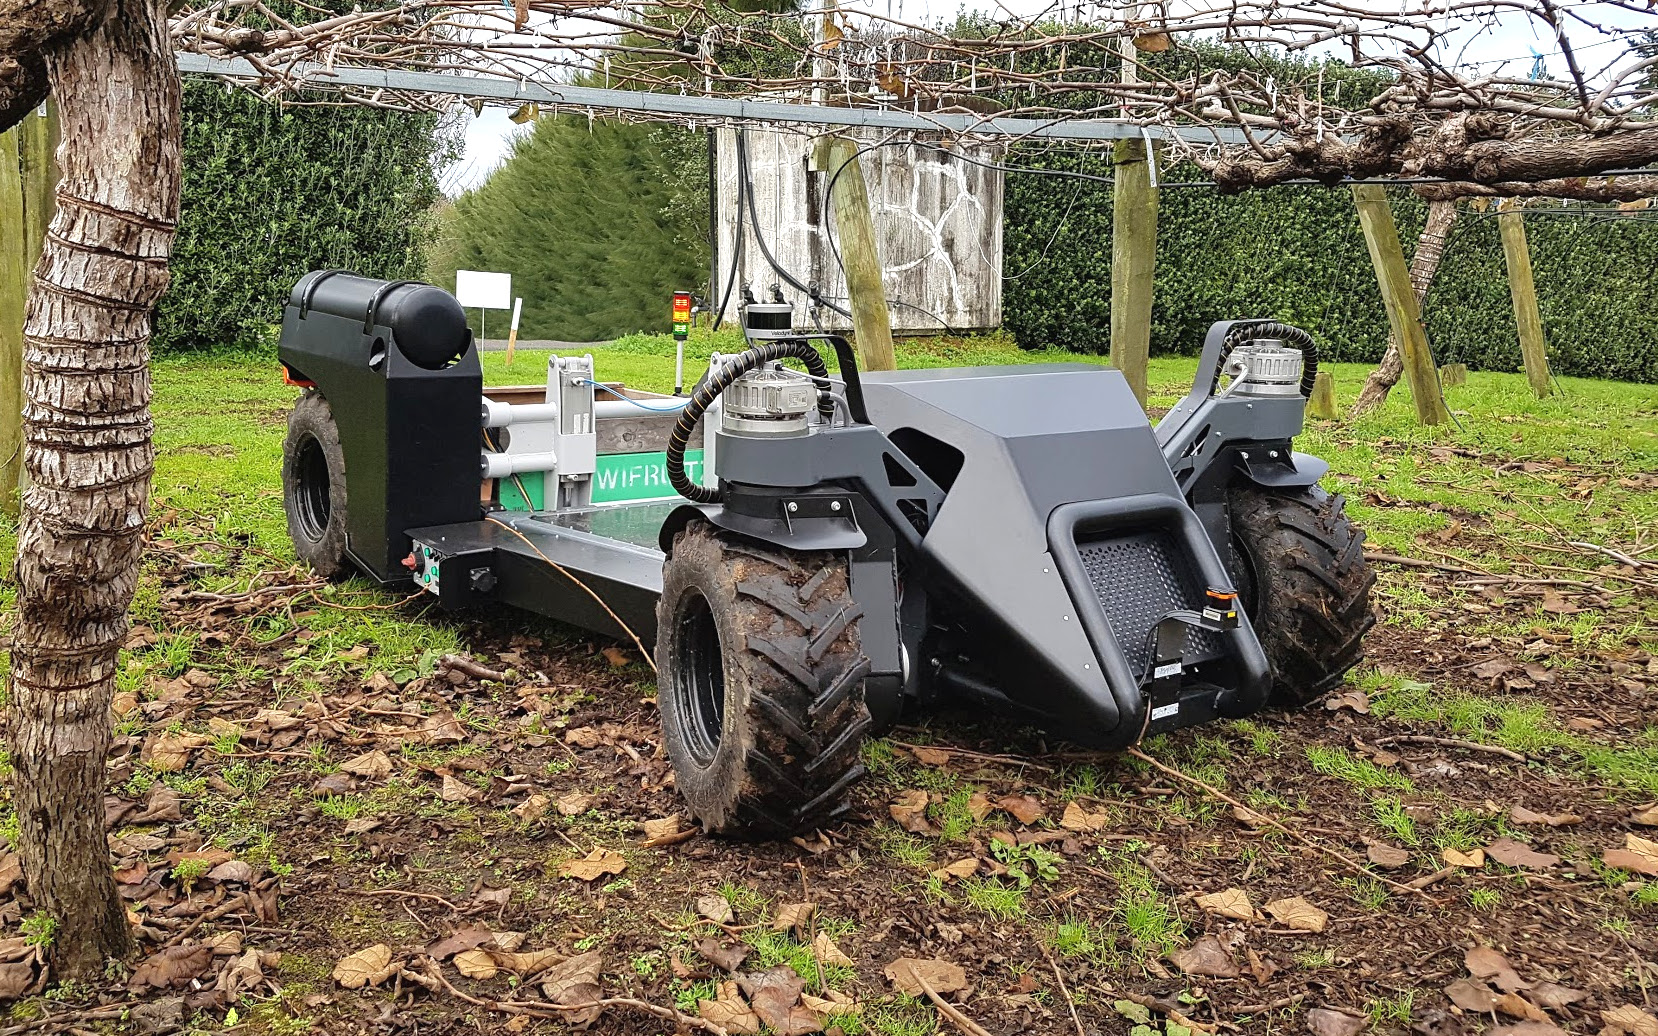
\includegraphics[width=\linewidth]{imgs/photos/suzy_general.jpg}
        \caption{
            The presented platform driving through a pergola style kiwifruit orchard during winter months.
        }
        \label{fig:suzy}
    \end{figure}


\section{Related Work}
\label{sect:review}

        The introduction of computers and digital camera technology during the 1980s sparked research into autonomous vehicles for agricultural use \citep{Li2009}.
        When publishing details of an autonomous vehicle in 1998, Tillett et~al.\@ cite difficulties dealing with variability in lighting and the environment as the reason no commercial vehicles were available at the time \citep{Tillett1998}.
        Their vehicle combined wheel encoders, a compass, and accelerometers for odometry information.
        It also featured a camera based row guidance system.
        The system as a whole was capable of spraying individual plants whilst driving autonomously at \SI{0.7}{\meter\per\second} (\SI{2.5}{\kilo\meter\per\hour}).
        While their purpose built experimental vehicle proved capable of row following and targeted spraying, it was not designed for modularity.


        Four years later, two autonomous vehicles designed for weed mapping and control in open field crops were presented \citep{Pedersen2002,Astrand2002}.
        These platforms had relatively simple chassis and drive systems as they were both at a prototype stage, i.e., neither were designed to carry heavy payloads.
        The first vehicle, presented by Åstrand \& Baerveldt, featured: two-wheel steering, two-wheel drive, a camera based row guidance system, batteries, a combustion engine, and an air compressor.
        While its appearance was basic, it contained most of the functionality required for use with modularised fruit handling modules.
        The second unit, described by Pedersen et~al.\@, was four-wheel drive with two-wheel steering and used satellite navigation as its primary navigation input.
        It was battery powered only and lacked any sort of row guidance sensor or power generation unit.
        The authors found that row-crop based navigation using satellite navigation alone was not practical and proposed the integration of a row-guidance sensor in their next design.
        They also proposed a revised drive system with four-wheel steering.% and a Controller Area Network (CAN) bus for low-level system communication as opposed to using serial links.

        Two years later, the revised design proposed by \cite{Pedersen2002} was presented by \cite{Bak2004}.
        Its drive system was modularised with four identical drive/steering modules mounted to the chassis.
        This revised chassis featured a three-point suspension system, which ensured all four wheels stayed in contact with the ground.
        The system also incorporated the row-guidance sensor as proposed in earlier work, as well as a Real-Time Kinematic enabled GPS receiver (RTK-GPS), fibre optic gyroscope, compass, and wheel encoders.
        The authors noted that the control strategy for the four independently controlled wheels was ``non-trivial''.
        While much more developed than the previous work of \cite{Pedersen2002}, the platform was not designed to: carry heavy payloads, operate in the absence of satellite navigation, or power itself beyond its battery capacity.

        In 2009, details of BoniRob were published by \cite{Ruckelshausen2009}.
        Similar to the previous unit presented by \cite{Bak2004}, it featured a gyroscope, RTK-GPS receiver, and four-wheel steering.
        However, it introduced the use of both single-plane and multi-layer laser range scanning, known as lidar, for perception and row detection.
        A \SI{2.8}{\kilo\watt} petrol engine could also be mounted to the chassis, additional to its on-board batteries.
        It was capable of carrying a \SI{150}{\kilo\gram} payload in its dedicated module space.
        What made BoniRob particularly interesting was its ability to alter its track-width by actuating the legs to which its wheels were mounted.
        Like the robots before it, BoniRob was designed for use on open-field crops.
        During the previous year, some of these authors published details of a much simpler robot named `Weedy' \citep{Klose2008}, also an open-field crop based sensing platform.
        BoniRob represents the first of the more general-purpose platforms designed to carry modularised payloads.

        Most recently, \cite{Bawden2017} published details of their field-crop robot -- Agbot~II.
        For locomotion it uses two driven wheels in a differential drive configuration with castor wheels for support.
        It is battery powered and designed to autonomously return to a shipping container with a built-in solar powered charging station.
        The vehicle is made of two side modules bridged by a modular centrepiece containing instrumentation.
        The side modules contain the drive system, whereas the centrepiece is designed to be specific to the application.
        As with all of the vehicles previously reviewed, its payload carrying capabilities are limited to ground facing modules, e.g., soil inspection and weeding.

        Of particular relevance, is the earlier work of Scarfe et~al.\@ on an autonomous kiwifruit picking robot \citep{scarfe2009, Scarfe2012}.
        That work involved the creation of a hydraulically driven platform, with two-wheel steering and four-wheel drive.
        Four fruit-harvesting arms and a bin-lifting mechanism were also integrated.
        While that platform was designed to navigate through kiwifruit orchards autonomously, its ability to do so was not tested due to an outbreak of \textit{Pseudomonas syringae pv. actinidiae} (PSA), which closed access to kiwifruit orchards.
        The platform had a petrol engine and made use of camera and lidar based row guidance sensors.
        It had sufficient carrying capacity for other roles, however it lacked modularity -- restricting its use to kiwifruit harvesting.

        With the exception of the platform presented by \cite{Scarfe2012}, all of the reviewed platforms were designed for use with open-field crops.
        None were designed for harvesting operations and therefore were not capable of carrying bins.
        Referring back to the statement from \cite{Ruckelshausen2009} that ``the application itself should be of comparably low complexity'', one can see why research thus far has focused on simpler tasks such as inspection or weeding.
        However, once designs move past these applications it becomes necessary to accommodate other shared requirements.
        A fork-lift mechanism is general enough that most orchard related tasks can benefit from it.
        For example, during harvesting it can hold a fruit collection bin.
        During a pollination season it can hold the tank of liquid pollen solution.
        The ability to pick up a standard pallet has broad applications in and around orchards too.

        % \cite{Blackmore2007} envisaged significant reductions in production costs for agricultural robotics by repurposing parts already in use in the agricultural and automotive industry.
        % High-power AC motor controllers are one such component which are increasingly being used by automotive manufacturers.
        % Significant cost reductions are possible by using controllers designed for integration by automotive manufacturers as opposed to more general purpose controllers.
        % While not a physical component, the CAN bus is another example of technology borrowed from the automotive industry.
        % Most of the more recent platforms made use of this for low-level communication.
        Reported use of GNSS systems indicate that they are not suitable for navigating row based crops on their own.
        With regards to the use of RTK based GNSS guidance, Slaughter et~al.\@ points out the trade-off of requiring an ``unobstructed `view' of the sky from all parts of the field'' \citep{Slaughter2008}.
        % \cite{Durrant-Whyte2005} describe one failure mode of GPS being multipath signal propagation caused by nearby foliage or the geometry of the land itself.
        \cite{Li2009} conclude that the use of either GPS and machine vision, or GPS and lidar will become a development trend.
        Based on the increased reception requirements, we discount the use of RTK based systems, but still consider the use of general purpose GNSS receivers as a navigation input.

\section{Platform Design}
\label{sect:design}
        \begin{figure}[htb]
            \centering
            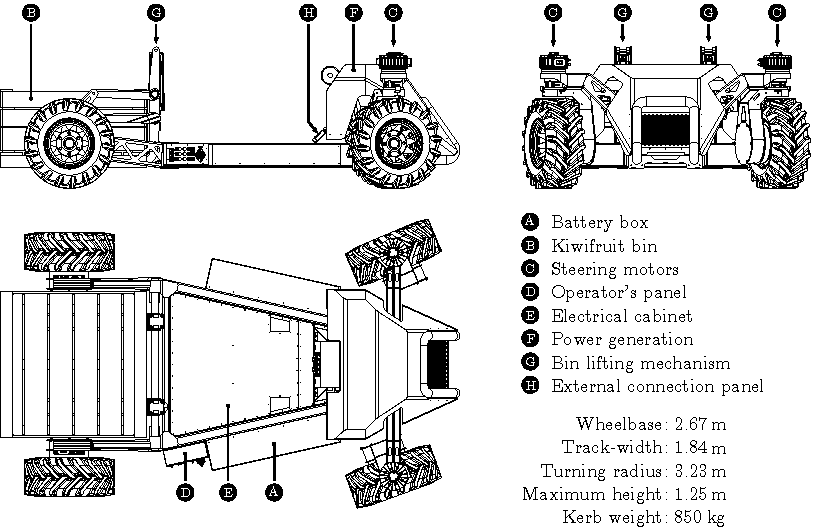
\includegraphics[width=\linewidth]{imgs/profile_views/AMMP-All-Labelled.pdf}
            \caption{Profile drawings of the robotic platform with kiwifruit bin.}
            \label{fig:AMMP}
        \end{figure}

        The vehicle's design is mostly influenced by the need to carry modularised robotic systems and fruit bins.
        Existing commercial platforms suitable for use in horticulture already exist, such as the Warthog from ClearPath Robotics, but the maximum payload, battery life, and vehicle geometry make them unsuitable for kiwifruit harvesting.
        The mass of robotic modules for pollination or harvesting can be as much as \SI{600}{\kilo\gram} and a bin of kiwifruit adds an additional \SI{400}{\kilo\gram}.
        The canopy height in typical commercial orchards range from \SI{1.4}{\meter} to \SI{1.7}{\meter}, so the vehicle must also have a low profile.
        Modules carried by the platform require clearance from the canopy in addition to the height they occupy themselves.
        To maximise the space available to these modules the platform must be low-slung at the point they attach.
        Figure~\ref{fig:AMMP} illustrates the platform's design, with module area allocated between markers `G' and `H' in the side-view (top left).
        The top surface of the chassis in this region sits \SI{360}{\milli\meter} above the ground.

        \begin{figure}[htb]
            \centering
            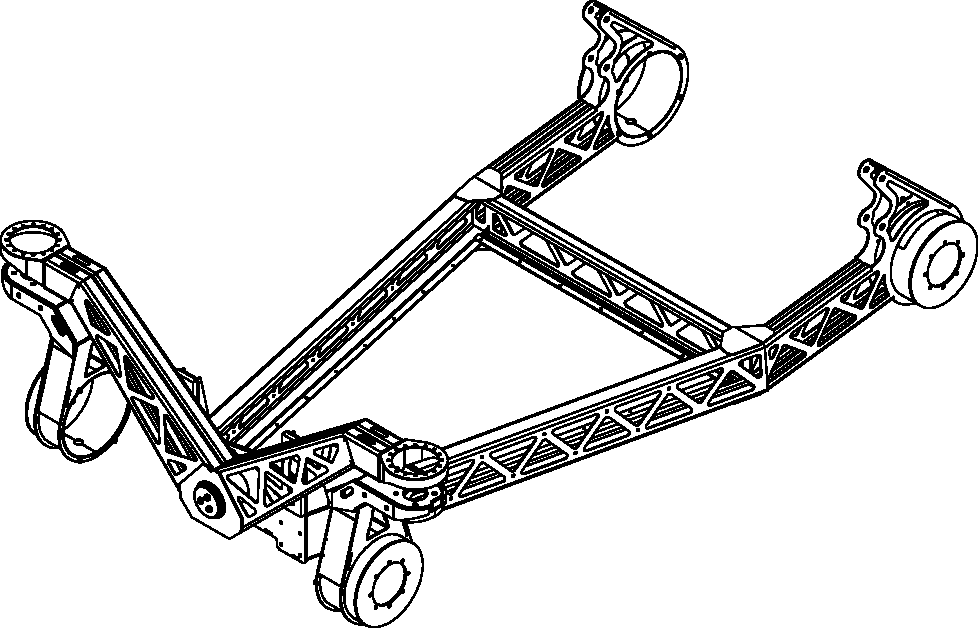
\includegraphics[width=0.6\linewidth]{imgs/profile_views/AMMP-Chassis-1-20.pdf}
            \caption{Drawing of the vehicle's chassis showing front pivot mechanism and steering linkages. The laser-cut and folded structure has a total mass of \SI{190}{\kilo\gram}.}
            \label{fig:AMMPChassis}
        \end{figure}

        The chassis is assembled from sections of \SI{3}{\milli\meter} laser-cut and folded mild steel.
        The sections are welded together on jigs, also made from laser-cut and folded steel, before being powder coated and assembled.
        Much of the folded chassis structure contains triangular cut-outs, reducing weight while having minimal impact on rigidity.
        Finite element analysis was used during the design phase to help identify areas needing to be strengthened and areas where material could be removed.
        This helped to ensure the platform meets its target load capacity of \SI{1000}{\kilo\gram}, while the bare chassis weighs only \SI{190}{\kilo\gram}.
        A drawing of the chassis is shown in Figure~\ref{fig:AMMPChassis}.

        Bin lifting forks occupy the area between the rear wheels.
        Fuel and compressed air tanks sit over the right-hand rear wheel, which can be seen in Figure~\ref{fig:suzy}.
        The bin lifter is actuated by two vertically mounted double-acting pneumatic cylinders (SMC CP96D100-320) which are controlled by a pneumatic valve block.
        Each cylinder is capable of exerting \SI{4700}{\newton} at \SI{600}{\kilo\pascal} or \SI{6300}{\newton} at \SI{800}{\kilo\pascal}.


    \subsection{Steering}
    \label{sub:steering}

        The steering geometry is Ackermann based, with the front two wheels being actuated by brushless AC motors (Heinzmann PSM G100).
        These motors can generate \SI{7.32}{\newton\meter} of torque with a maximum angular velocity of \SI{3000}{rev\per\minute} and are rated at \SI{2.3}{\kilo\watt}.
        Their outputs are fed through fixed-ratio planetary gearboxes with a 64:1 reduction, increasing torque to \SI{470}{\newton\meter} while reducing the maximum angular velocity to \SI{47}{rev\per\min}.

        Torque requirements for the steering motors are based on a static friction scenario with the vehicle loaded with a \SI{1000}{\kilo\gram} mass, sitting on concrete.
        This is described by the following equation:
        \begin{equation}
        \label{eqn:steer_torque}
        \tau = W u \sqrt{\frac{B^2}{8} + E^2}
        \end{equation}
        where $\tau$ is the torque required to break static friction, $W$ is the force transmitted through a wheel, $u$ is the coefficient of friction, $B$ is the nominal width of the tyre, and $E$ is the offset between the tyre's contact surface and its axis of rotation.
        The axis of rotation on the vehicle lies directly through the centre of the tyre, meaning $E=0$.
        % As the axis of steering rotation lies directly through the centre of the wheel, $E=0$.
        A value of 0.75 was used as the coefficient of friction as a best guess representation of a tractor-grip tyre on dry concrete.
        The mass of the vehicle (\SI{800}{\kilo\gram}), plus payload (\SI{1000}{\kilo\gram}), and fuel (\SI{60}{\kilo\gram}) adds to \SI{1860}{\kilo\gram}.
        Allowing for uneven weight distribution on the vehicle and a safety margin, the per-wheel mass supported is \SI{500}{\kilo\gram}, or a weight of \SI{4900}{\newton}.
        The tyre width is \SI{0.28}{\meter}.
        By combining these values, as per Equation~\ref{eqn:steer_torque}, a torque of \SI{388}{\newton\meter} is required to overcome static friction when actuating the steering motors.

        Actuating the steering wheels independently removes the need for mechanical linkages between them, allowing for more extreme steering angles and a simpler mechanical design.
        Both steered wheels have the freedom to rotate \SI{330}{\degree}, artificially limited by mechanical stops.
        At the tightest steering angle of \SI{90}{\degree}, the centre-point of the turn is located at the midpoint of the rear wheels.
        The turning radius in this case should be equal to the distance between the front bumper and the rear wheels (\SI{3.18}{\meter}).

        Implementing a four-wheel steering system would shift the pivot point to the vehicle's centre, roughly halving the turn radius, but this was deemed unnecessary.
        Headlands in kiwifruit orchards are sized for tractors with much larger turning radii than that of our platform.
        The use of a two-wheeled steering system removes the need to develop the ``non-trivial'' control strategies mentioned by \cite{Bak2004}.
        It also increases the usable area at the rear of the vehicle by removing the need for clearances around actuated wheels.
        A skid steer system was expected to cause ground damage to a level considered unacceptable to orchard owners when carrying heavy loads.

        The steering motors have incremental encoders, but no means of absolute positioning built-in.
        This means that the front-wheel angles must aligned before use.
        A homing sequence at boot-up is used to find an absolute angle as a reference point for relative rotation data.
        Inductive proxy sensors are used as a means of detecting the position of the wheels during this sequence.

    \subsection{Drive system}
    \label{sub:drive}
        The vehicle features a three-point suspension system, as was used by~\cite{Bak2004}, to ensure all wheels remain in contact with the ground.
        It uses a pivoting front axle to do this, depicted in Figure~\ref{fig:AMMPChassis}.
        As the operating speed for the vehicle is \SI{1.39}{\meter\per\second} (\SI{5.0}{\kilo\meter\per\hour}), the tyres alone were expected to provide sufficient shock absorption.

        % \begin{figure}[htb]
        %     \centering
        %     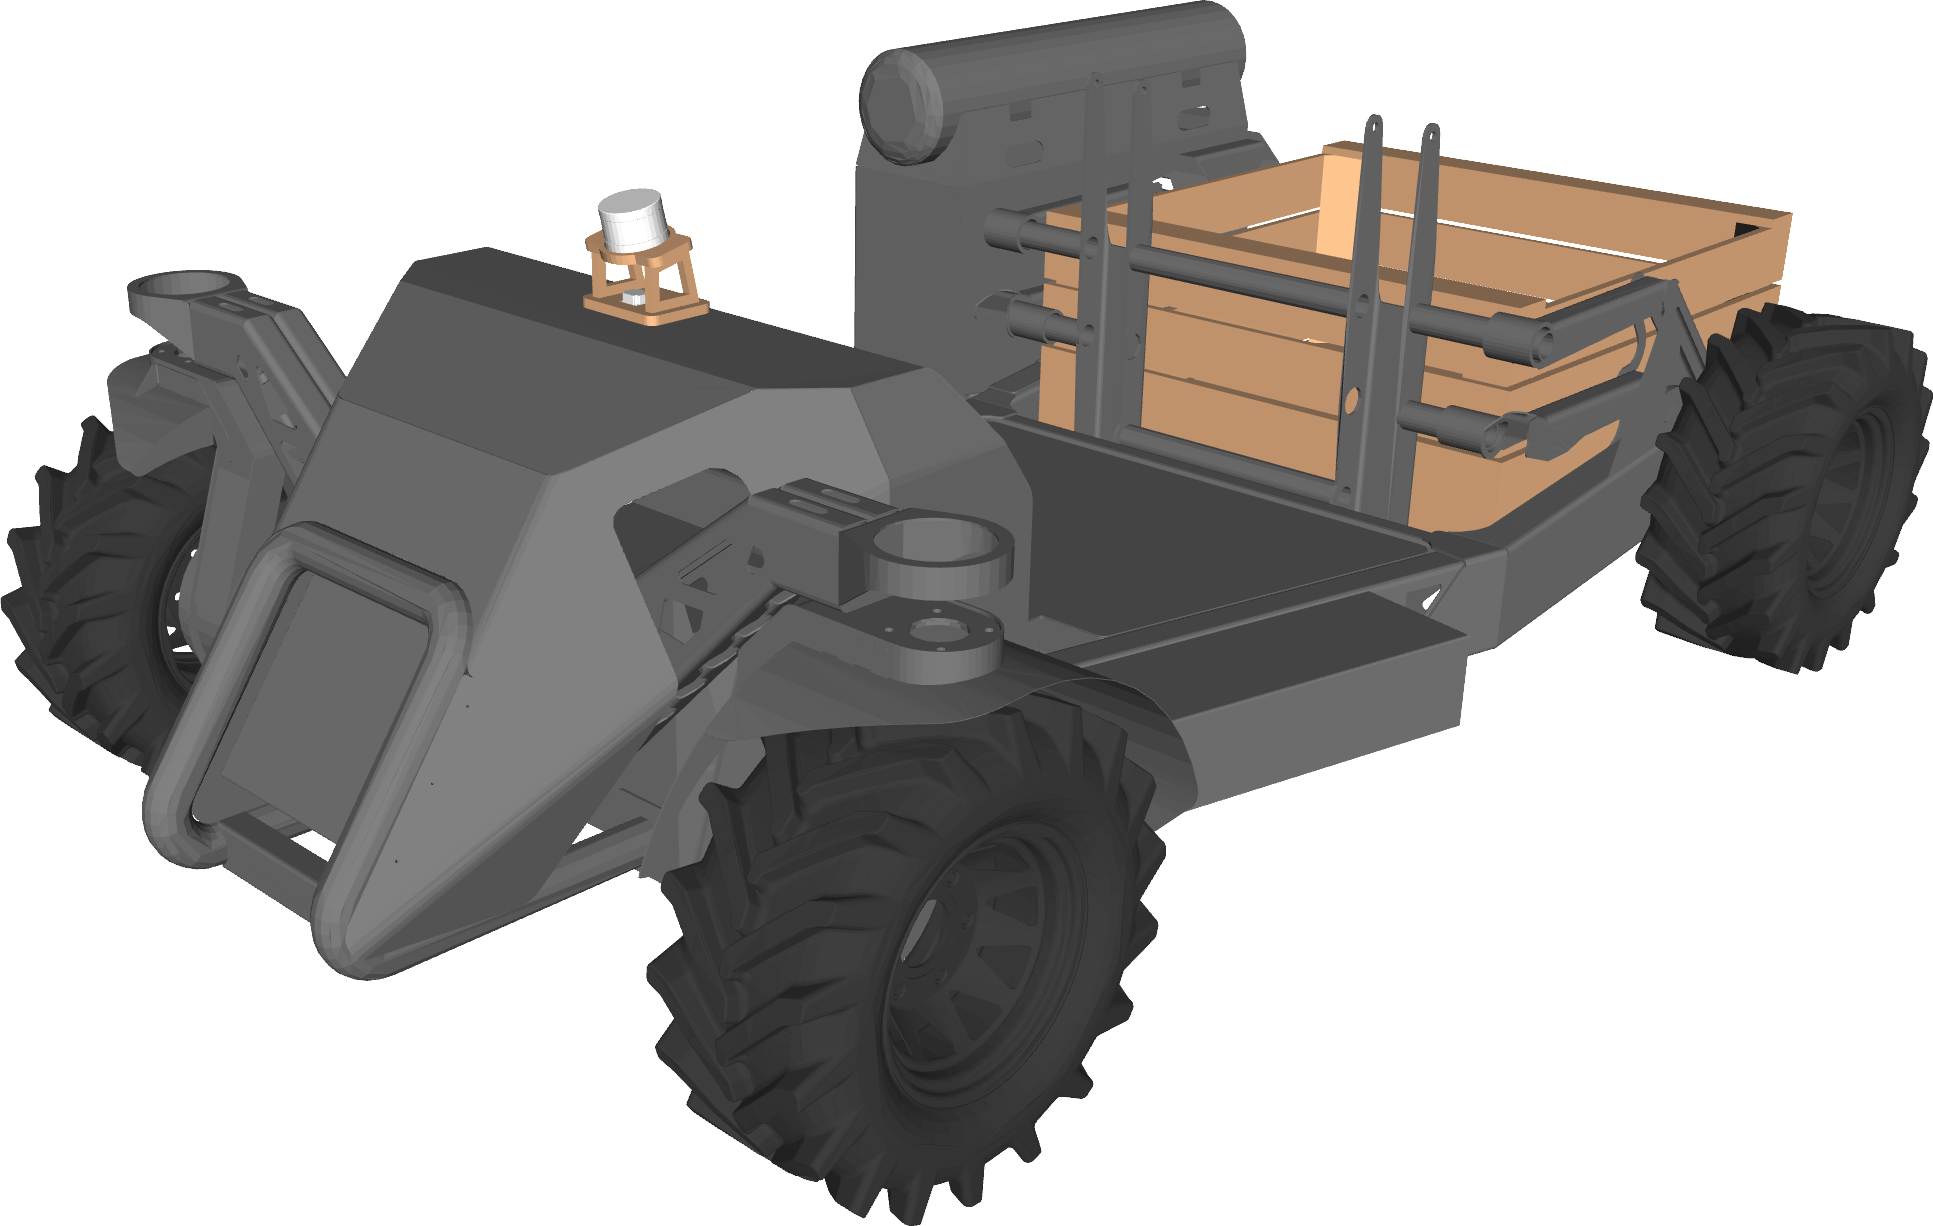
\includegraphics[width=0.8\linewidth]{imgs/photos/RVIZ.png}
        %     \caption{3D Model showing placement of the lidar and IMU at the front of the vehicle.}
        %     \label{fig:rviz}
        % \end{figure}

        % Potentially useful picture above
        %%% Mark: Editing checkpoint (from beginning)

        Performance requirements for the vehicle's traction system during up-hill acceleration while under load were calculated as follows:
        \begin{align}
        \label{eqn_f_rolling}
        F_{rolling} &= C_{rr} \times m\\
        F_{grade} &= m \times G \times \sin(\alpha)\\
        F_{accel} &= m \frac{\Delta v}{t}\\
        \label{eqn_f_accel}
        F_{total} &= F_{rolling} + F_{grade} + F_{accel}
        \end{align}
        Where $F_{rolling}$ is the force due to rolling-resistance; $F_{grade}$ is the grade (or incline) force; and $F_{accel}$ is the force required for mass acceleration.
        A rolling-resistance coefficient ($C_{rr}$) of 0.04 was chosen based on values found in an automotive handbook \citep{RobertBoschGmbH2002}.
        It represents the case of a pneumatic tyre on medium-hard soil.
        Other variables used are: a vehicle mass ($m$) of \SI{1900}{\kilo\gram}, slope angle ($\alpha$) of \SI{20}{\degree}, velocity change ($\Delta t$) of \SI{2.78}{\metre\per\second} (\SI{10}{\kilo\meter\per\hour}), and an acceleration time ($t$) of \SI{6}{\second}.
        Putting these values through Equations \ref{eqn_f_rolling}--\ref{eqn_f_accel} gives a total force requirement of \SI{7.99}{\kilo\newton}.
        On a per-wheel basis this is \SI{2.0}{\kilo\newton}, or \SI{729}{\newton\meter} when taking the wheel radius ($r$) of \SI{0.365}{\meter} into account.
        Required traction power ($P$) is then calculated as follows:
        \begin{align}
        \label{eqn_f_power}
        \omega &= 2 \pi \times \frac{v}{2 \pi r} = \frac{v}{r}\\
        P &= \tau \omega
        \end{align}
        where $\omega$ is the angular velocity of a wheel, $v$ is the vehicle velocity, and $\tau$ is torque.
        At a velocity of \SI{2.78}{\meter\per\second} (\SI{10}{\kilo\meter\per\hour}), the calculations give a power requirement of \SI{5.55}{\kilo\watt} per wheel.

        The selected motors are hub-mounted permanent magnet brushless AC motors with integrated 40:1 fixed-radio planetary gearboxes (Heinzmann PSM-G120).
        Each motor is rated for \SI{6.4}{\kilo\watt} at \SI{96}{\volt} with a maximum angular velocity of \SI{3000}{rev\per\min} and torque of \SI{20.4}{\newton\meter}.
        At the output of the gearbox the torque jumps to \SI{816}{\newton\meter} while the angular velocity drops to \SI{75}{rev\per\minute}; giving the platform a top speed of \SI{2.86}{\meter\per\second} (\SI{10.3}{\kilo\meter\per\hour}).

        In total there are seven brushless AC motors on-board the platform: four drive motors, two steering motors, and a motor used for electrical power generation.
        Each are connected to individual AC motor controllers (Sevcon Gen4 DC Size 4).
        These controllers are available in four bus voltage options: 24-36V, 36-48V, 72V-80V, and 96V-110V.
        The six motors used for traction and steering are together capable of consuming \SI{30.2}{\kilo\watt}.
        With a \SI{48}{\volt}DC bus this would equate to a current draw of \SI{630}{\ampere}.
        As \SI{24}{\meter} of cabling is required to connect the motors and controllers to a common point on the vehicle, a \SI{96}{\volt}DC bus was used to reduce the required gauge of that cable.


    \subsection{Power Distribution}
    \label{sub:power}
        The system bus connects the batteries and generator to motor controllers and on-board power converters.
        A series of heavy-duty contactors (TE Connectivity Kilovac LEV200) control each device's connection to the bus, as well as the bus's connection to the power source.
        Figure~\ref{fig:power_system_diagram} illustrates power-distribution on the platform.

        \begin{figure}[htb]
            \centering
            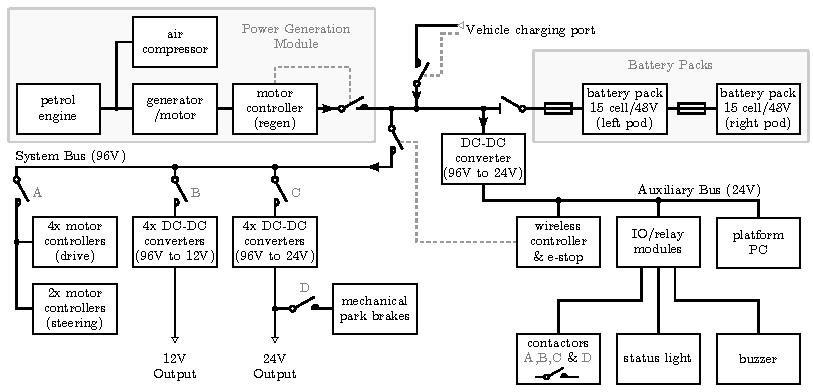
\includegraphics[width=\linewidth]{imgs/system_diagram/full-system-diagram_v1.pdf}
            \caption{Power distribution system diagram. Dashed lines in grey indicate control lines to contactors.}
            \label{fig:power_system_diagram}
        \end{figure}

        Two battery modules attached to the sides of the chassis each house fifteen lithium-iron-phosphate (LiFePO$_{\text{4}}$) batteries connected in series.
        Together, the batteries (Winston/Thundersky WB-LYP90AHA) provide a nominal bus voltage of \SI{96}{\volt} and a total electrical capacity of \SI{8.64}{\kilo\watt\hour}.
        The battery packs were manually `bottom-balanced' before being fitted and no cell-level voltage monitoring is present.
        Maximum and minimum pack voltages were established by monitoring individual cells during charging and discharging.
        At the point that any individual cell exceeds a safe maximum/minimum threshold, the respective maximum/minimum pack voltage is determined.

        A hermetically sealed disconnect switch (Gigavac HBD41) isolates the batteries from the system.
        Once closed, an auxiliary \SI{24}{\volt} bus becomes active that powers components required to bring the rest of the system on-line.

        A power generation unit comprised of a petrol engine (Honda GX-690), air compressor (Rotorcomp NK-1), and electrical generator is housed at the front of the vehicle.
        The drive shafts of these units are connected via pulleys and a heavy-duty timing belt.
        The engine, compressor, and alternator are controlled and monitored by a micro-controller based control board.
        This board connects to the Platform PC via the system CAN bus.
        The engine is capable of producing \SI{16}{\kilo\watt}, where up to \SI{9.6}{\kilo\watt} is converted to electrical power (limited in software) and \SI{4.0}{\kilo\watt} is converted to pneumatic power.
        The system maintains a pneumatic tank pressure of \SIrange{600}{800}{\kilo\pascal}.

        Electrical generation is done with a brushless AC motor/generator (Heinzmann PMSG-150) connected to the same model of motor controller used with the drive system.
        This motor was a larger variant of those used for traction and steering, minus the gearbox.
        Its controller was configured only to have regenerative braking functionality, i.e., power could not be applied to the motor.
        This configuration allowed the system to control the rate of power generation by commanding braking effort from the controller.
        The controller provides voltage and current limits as well as the ability to reduce output as the batteries become charged.
        These settings provide all the functionality of a general purpose battery charger, making this a cost effective and versatile charging solution.
        Electrical energy from the power generation unit is fed to the batteries in a series-hybrid configuration.
        An external charging port is also fitted to allow charging of the batteries directly.

        A fuel tank is fitted over the rear right-hand wheel (visible in Figure~\ref{fig:suzy}).
        It can hold \SI{60}{\litre} of petrol, allowing the vehicle to operate continuously for over \SI{24}{\hour}.
        On-board DC-DC converters deliver \SI{2.8}{\kilo\watt} at \SI{12}{\volt}DC, \SI{3.8}{\kilo\watt} at \SI{24}{\volt}DC, and \SI{3.5}{\kilo\watt} at \SI{240}{\volt}AC, simultaneously.
        A connection panel at the front of the module mounting area houses the weather-sealed plugs through which these outputs are accessible.


    \subsection{Communications Architecture}
    \label{sect:architecture}

        \begin{figure}[htb]
            \centering
            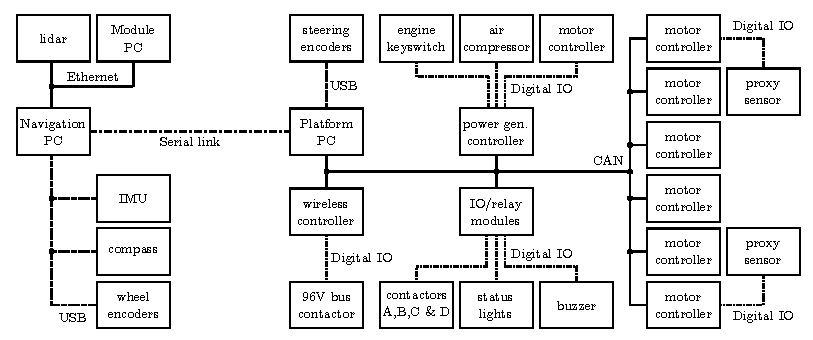
\includegraphics[width=\linewidth]{imgs/system_diagram/diagram_v5.pdf}
            \caption{
                Communications level system diagram showing types of links between devices.
                Devices on right-hand side of the serial link are mechanically integrated into the vehicle, whereas those on the left are modular and can be removed.
            }
            \label{fig:system_diagram}
        \end{figure}

        The platform is centrally controlled by an x86 based small-form-factor PC (Intel NUC) running Ubuntu 16.04 server edition, referred to as the ``Platform PC''.
        This computer communicates with most sub-systems via a CAN bus interfaced using a USB adaptor (IXXAT USB-to-CANV2).

        A second, externally mounted, computer is responsible for higher level control of the vehicle.
        It is used to connect to navigation sensors, send drive commands to the platform, and perform processing tasks relevant to autonomous navigation.
        It too is an x86 based PC running Ubuntu, but uses a commodity motherboard with a discrete graphics card (Nvidia GTX 1080Ti).
        The graphics card is used to accelerate neural network algorithms and some image processing functions.
        An Ethernet network connects this PC to the mounted payload modules, while a RS422 serial link is used to communicate with the Platform PC.
        Figure~\ref{fig:system_diagram} illustrates this arrangement.

        In addition to the drive commands generated by the Navigation PC, a wireless controller (HBC Radiomatic Eco) lets the operator issue drive commands via joystick.
        The controller's receiver module contains relays that are directly controllable from the remote control.
        All inputs from this controller are also broadcast onto the CAN bus and read by software nodes on the Platform PC.
        The remote control has two joystick inputs, two selector switches, four buttons, and an emergency-stop switch.
        The emergency stop switch is connected to the \SI{96}{\volt} bus contactor via relay outputs from the receiver unit.
        If this switch is closed during operation, or the controller goes out of range, power to the bus is cut within \SI{500}{\milli\second}.
        This engages the mechanical park brakes, removes all tractive effort from the motors, and de-powers mounted modules.

        The open source Robot Operating System (ROS) is used to facilitate communication between computers and software nodes running within each computer.
        Nodes written using this framework follow either a publish-subscribe or service-client pattern.
        To maximise code reusability, each device on the platform has its own ROS-compatible node dedicated to publishing device data or subscribing to generated device commands.
        Interface adapters, motor controllers, wireless controllers, lidar, and encoders are examples of devices on the platform with dedicated interface nodes.
        Nodes can be written in either C++ or Python and can be used simply to transform or perform calculations on data while passing it between other nodes.
        For instance, as shown in Figure~\ref{fig:system_diagram_software}, an `Ackermann kinematics' node transforms a steering vector into individual wheel velocity and position/angle outputs.
        Among other things, ROS offers the ability to monitor and record all communication passing through it which can be replayed and examined later.

        The manufacturer's configuration of the motor controllers require them to be interfaced using a combination of analogue and digital inputs.
        For example, the accelerator and steering inputs are controlled by potentiometers actuated by the vehicle's driver.
        However, the controllers also provide an option for a multi-motor vehicle configuration.
        In this configuration, the analogue inputs fed into a master controller are relayed to a second controller over a CAN interface.
        This interface is configured using a proprietary tool and is not intended for use other than between controllers configured with their software.
        By observing the communication protocol between a master and slave in operation, it was possible to implement a master node in software that runs on the Platform PC.
        With this, all motor controllers on the platform are programmed as slave devices.
        This allows them to accept drive commands via CAN interface, allowing them to be directly controlled by ROS nodes.

        Relay modules allow the Platform PC to toggle power to on-board power supplies, motor controllers, park-brakes, and lights.
        They also monitor the timing of synchronisation messages transmitted by the Platform PC onto the CAN bus.
        These synchronisation messages are configured to occur every \SI{20}{\milli\second} as an indication that the system is running as expected.
        Once a relay module detects an absence of these messages for \SI{100}{\milli\second} or longer it enters an error state.
        This causes the motor controllers and on-board power supplies to be shut-off and the park-brakes to be engaged.
        Synchronisation message monitoring is used as a fail-safe mechanism to ensure the system is promptly shut-down if the Platform PC fails.

        The open source simulation package Gazebo was used to simulate the vehicle's steering geometry with input from a game-pad.
        This revealed issues that were resolved before implementation on the physical hardware.
        It also provided the opportunity to tune control parameters, such as steering sensitivity, while reducing the time to test.

        \begin{figure}[htb]
            \centering
            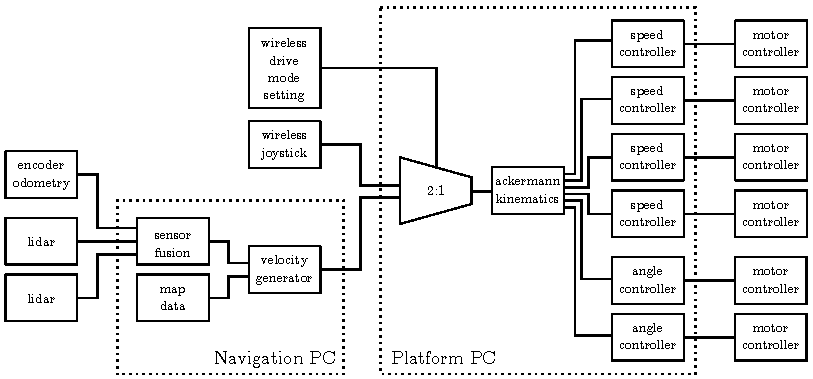
\includegraphics[width=\linewidth]{imgs/system_diagram/software_v2.pdf}
            \caption{Simplified diagram showing connectivity between ROS nodes used for manual and autonomous platform control.}
            \label{fig:system_diagram_software}
        \end{figure}


\section{Navigation Sensor Selection}
\label{sect:sensors}
    The choice of sensors incorporated into a vehicle determines which algorithmic approaches are available for navigation and object detection.
    Lidar, cameras, and GNSS receivers have been considered.
    Each sensor's ability to capture relevant data is evaluated by in-orchard trials.

    Other sensors considered for inclusion are outlined in Table \ref{table:sensor_comparison} along with their associated issues.
    Factors considered were the strengths and weaknesses in the context of orchard use, reported usage in literature, and availability at a suitable price.
    A review of previous works highlighted both lidar and 2D cameras as offering high functionality for navigation and object detection.
    Time-of-flight cameras are a compelling option based on a cost-benefit analysis; especially if cheaper units work outdoors in the presence of sunlight.
    Because localisation is such a key function, the performance of two GNSS receivers has also been evaluated.

    \begin{table}[htbp]
        \centering
        \footnotesize
        \begin{tabular}{ l l}

            \textbf{Sensor Type}      &\textbf{Common Issues} \\ \hline
            GNSS receiver              & Prone to signal loss from surrounding foliage\\  \hline
            Inertial Measurement Unit & Error accumulation and thermal drift\\ \hline
            Digital Compass           & Prone to disturbance by nearby metallic structures\\ \hline
            Encoder                   & Error accumulation \\ \hline
            Lidar                     & Reduced visibility in fog and heavy rain \\ \hline
            Time of Flight Camera     & Reduced visibility in sunlight, fog and heavy rain \\ \hline
            Camera                    & Reduced visibility in fog or direct sunlight \\ \hline
            Thermal Camera            & Reduced visibility in conditions of low thermal contrast\\ \hline
        \end{tabular}
        \caption{Sensor types considered for inclusion on the platform.}
        \label{table:sensor_comparison}
    \end{table}

    As the drive motors have built-in wheel encoders, basic odometry data is already available.
    Encoders on driven wheels will give false readings if wheel slippage occurs so are not be used for odometry alone.
    However, the data provided can still be used to assist with mapping, localisation, and provide velocity feedback.


    \subsubsection{In-orchard Camera Evaluation}
        \label{sect:camera_evaluation}

        Three types of camera were tested: time-of-flight, 3D stereoscopic, and traditional 2D cameras.
        Smaller platforms (Clearpath Husky and Adept MobileRobots Pioneer P3-AT) were used to gather data used for evaluation.
        Cameras were mounted \SI{0.8}{\meter} above the ground, roughly mid-way between the ground and the canopy, facing forward.

        The time-of-flight camera was a Basler TOF640-20GM-850NM.
        It provides range, intensity, and confidence data at a resolution of 640 by 480 pixels.
        This specific model was chosen as it had previously proved useful when collecting depth data of kiwifruit canopies.
        During that time it had been operated under a range of lighting conditions and exhibited minimal occurrences of data loss.
        In those conditions the camera was mounted with its principal axis aligned vertically, pointing upwards to the canopy.
        However, subsequent testing with the camera mounted with its principal axis aligned horizontally revealed significant data loss in both sunny and overcast conditions.
        This is thought to be the result of two factors.
        The first is a lower reflectivity of objects in view of the camera when facing forwards, as opposed to facing up at a leafy canopy.
        The second is due to a dramatic increase in distance between the camera and the scene's subject matter.
        As the camera relies on active illumination of the scene, its ability to detect that illumination amongst ambient light will drop sharply with distance.

        The 3D stereo camera tested was an Intel RealSense R200.
        It combines a stereo pair of infra-red cameras with a colour camera.
        Additionally, it features an infra-red projector as a means of adding texture to objects in its field of view to assist with stereo processing.
        The appealing characteristics of this sensor were its low cost and its claim of being long-range and able to work outdoors.
        However, in both overcast and sunny conditions it suffered from a \emph{complete} loss of range data.
        This appeared to be the result of ambient light interfering with the infrared projector’s signal.

        Traditional, 2-dimensional, cameras trialled were the Basler Dart daA1600-60uc, Flir CM3-U3-13S2C-CS, and a Logitech C920 web-camera; images shown in Figure~\ref{fig:cameraComparison}.
        The Logitech C920 suffered from significant motion blur that, being a consumer grade web-camera, was not surprising.
        It also lacked the functionality of a hardware trigger and sent images with significant latency, measured at \SI{150}{\milli\second}.
        The Basler and Flir cameras both produced images of sufficient quality and featured hardware triggering.
        The Basler camera had a USB3 interface and an average image transfer time of \SI{14}{\milli\second}.
        The Flir camera had a USB2 interface and an average image transfer time of \SI{65}{\milli\second}.
        The Basler offering was favoured for its later model image sensor, simpler software interface, and lower-latency.

        \begin{figure}[htb]
            \centering
            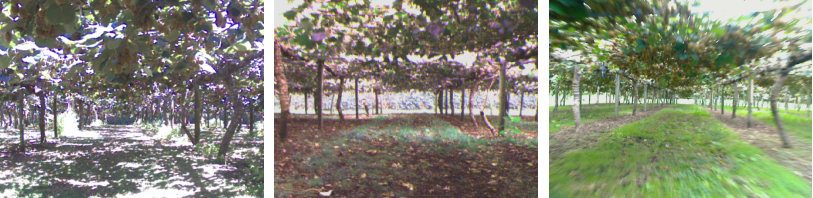
\includegraphics[width=\linewidth]{imgs/camera_comparison/camera_comparison.pdf}
            \caption{
                Example images captured from trialled 2D cameras.
                Basler Dart daA1600-60uc (left), Flir CM3-U3-13S2C-CS (centre), Logitech C920 web-camera (right).
            }
            \label{fig:cameraComparison}
        \end{figure}

        Both the time-of-flight and 3D stereoscopic camera systems were deemed unsuitable based on the occurrences of data loss.
        Images from the industrial 2D cameras (from Basler and Flir) were deemed suitable for object detection and classification.
        This was verified by processing the data using readily accessible detection algorithms such as convolutional neural networks.
        Using a pair of these 2D cameras it is also possible to build a stereoscopic pair.
        This provides the same functionality of the 3D stereoscopic camera from Intel, but without requiring the infra-red projector.
        Stereo pairs of industrial cameras have since proven useful on modularised harvesting and pollination modules for localising fruit and flowers, but were not tested for row following.


    \subsubsection{In-orchard Lidar Evaluation}
        Three lidar were evaluated, two single-plane and one multi-layer.
        The two single-plane lidar were the Hokuyo UTM-30LX and a SICK LMS111.
        The multi-layer lidar is a Velodyne VLP-16 which has 16 horizontal \SI{360}{\degree} layers separated over \SI{15}{\degree}.
        Data was collected from each device while driving through orchard rows with the sensor placed \SI{0.8}{\meter} above ground level.

        \begin{figure}[htb]
            \centering
            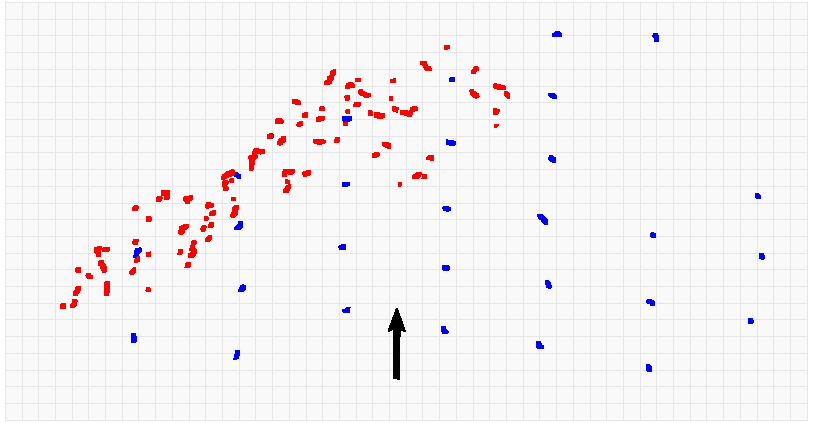
\includegraphics[width=\linewidth]{imgs/canopy_data/canopy_data.pdf}
            \caption{
                Data captured from a single plane lidar showing non-structural points reflected by the canopy (indicated by red markers) and structural points from tree trunks and posts (blue markers).
                The arrow indicates the position and heading of the platform at the time of capture.
            }
            \label{fig:canopyDataCloud}
        \end{figure}

        The intention was to use lidar as a means of detecting structure defining features of the orchard, such as posts, trunks and hedges.
        Detecting these features should allow for row boundary detection and general mapping and localisation.
        However, both single-plane lidar units produced clouds of unstructured data amongst the structured features; this is shown in Figure~\ref{fig:canopyDataCloud}.
        The cause was the lidar's scan plane intercepting with the above canopy whilst driving over convex terrain.
        Similarly, this issue arose on concave terrain when the plane intercepted with the ground.
        These situations are depicted in Figure~\ref{fig:concaveSlope}.

        \begin{figure}[htb]
            \centering
            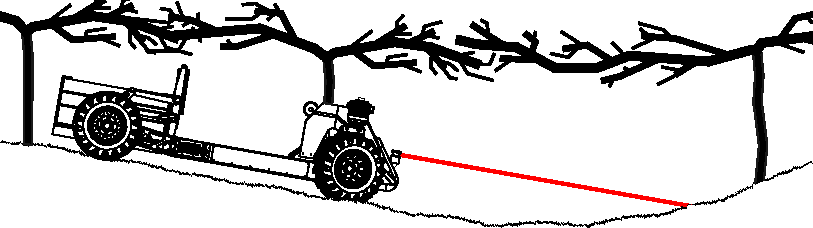
\includegraphics[width=\linewidth]{imgs/concave_slope/concave_slope_v4.pdf}
            \caption{
                On concave slopes the lidar scan plane meets the ground instead of striking row-defining features.
                The dashed line shows a horizontal plane coming from the the lidar.
                Dotted lines represent the most upper and lower layers from the multi-layer lidar.
            }
            \label{fig:concaveSlope}
        \end{figure}

        The issue was reduced by the use of a multi-layer lidar and post-processing the scan data.
        Having sixteen layers available meant it was possible to select a scan layer that gives the most useful viewing range.
        Referring again to Figure~\ref{fig:concaveSlope}, that would correspond to the dotted line above the horizontal (dashed) line which intercepts with a row defining feature (a tree trunk).

        It was decided that a multi-layer lidar would be best suited for navigation due to its ability to to see more distant features while driving on undulating ground.
        A single-plane lidar could still be used at short range as an independent channel of processing for redundancy or obstacle detection.

    \subsubsection{In-orchard GNSS Evaluation}
        Two GNSS receivers were evaluated: a Ublox Neo-M8N module and an OmniSTAR 5120VBS with AX0 series antenna.
        Both were connected to a single board computer (Beaglebone Black).
        The Ublox module was selected for its high sensitivity and internal low-noise amplifier.
        It was capable of receiving GPS, Galileo, GLONASS, and BeiDou GNSS signals concurrently.
        The OmniSTAR receiver was chosen for its external high-gain antenna (34 dB) which claims multi-path rejection.
        It was capable of receiving only GPS signals.

        The testing procedure first involved planning a path through a single row of a kiwifruit orchard.
        The receivers were then tested separately over the course of approximately two hours by walking them along the planned path.
        Before testing, each unit was powered up and given \SI{30}{\minute} to initialise in an open area near the kiwifruit orchard.
        During testing, each unit was walked slowly along the predetermined path with stops at each waypoint to provide time for a positional fix.
        The path was approximately \SI{500}{\meter} in length and took approximately \SI{15}{\minute} to complete, including stops at each waypoint.
        Way-points were spaced at intervals of \SI{5.5}{\meter} along the row.

        \begin{figure}[htb]
            \centering
            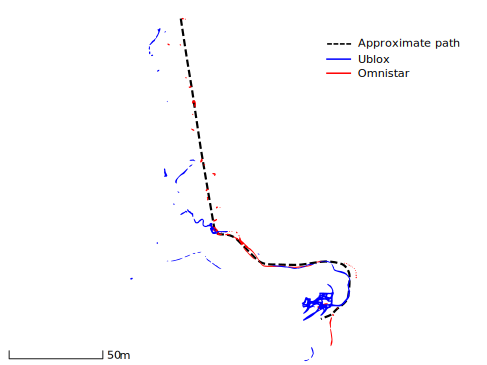
\includegraphics{imgs/gps_path/gps_path.pdf}
            \caption{
                Aerial view of the path taken through the test orchard and the captured GPS data.
                Dashes representing the approximate path are spaced at intervals of \SI{5.5}{\meter}.
            }
            \label{fig:gpsResults}
        \end{figure}

        The path followed, together with coordinates collected from the receivers, are presented in Figure~\ref{fig:gpsResults}.
        It should be noted that data has been recorded for the round-trip so represents two passes along the path.
        It was noticed during testing that the signal quality lights on both receivers regularly indicated a loss of signal.

        The Omnistar unit appears to track the approximate path well, but the data is sparse with regular loss of signal after entering the orchard.
        The Ublox unit collected more data, but was much less accurate.
        It may be possible to use a unit such as the Omnistar, which provided fewer but more accurate readings, as a sanity check for an approximate location within orchards.
        Overall, the units could not be relied on for localisation in this environment.
        These results indicate GNSS receivers with similar performance to those trialled are unsuitable for use in kiwifruit orchards.


\section{Autonomous Block Traversal}
\label{sect:autonomous}
    Two row following strategies were developed for implementation on the platform.
    Further details and results of each have been published separately.
    One method used multi-layer lidar to detect the trunks and posts of the orchard and follow a centre-line between them \citep{Bell2016}.
    The second method used a single camera combined with a convolutional neural network to segment features within the image.
    These features were: traversable space, tree-lines, and row-ends \citep{Bell2017}.
    A centreline was then fitted to the areas marked as traversable and used to generate a control vector.

    Both algorithms were developed on smaller, commercially available, test platforms while our larger platform was being built.
    A laptop (Dell E6410) with integrated graphics processor (Nvidia M5000M) was used on those platforms to process sensor data and generate drive vectors.
    Both approaches produced paths that led to reproducible row following behaviour.
    A method of conducting row-end turns was trialled on the Pioneer 3-AT robot using the lidar based approach.
    However, the platform's drive system lacked the power required to turn into rows on uphill slopes.

    To determine when the vehicle was at the end of a row, the multi-layer lidar was used to detect the absence of canopy in a volume above the front and to the sides of the vehicle.
    The camera based method was unable to detect this end-of-row condition which is necessary for initiating the turn.
    It also lacked the ability to locate obstacles, which is critical for our target platform due to its size and power.
    Finally, the lidar based approach required much less computational power to achieve similar performance.
    While it would be possible to combine the approaches, only the lidar based method was adapted for use on the target platform.

    Differences in geometry meant adjustments were needed when installing the sensors on the target platform.
    The multi-layer lidar was mounted horizontally above the front-right steering motor, visible in Figure~\ref{fig:suzy} and in Figure~\ref{fig:suzy_turning}.
    The smaller platforms used a skid-steer geometry, whereas our platform uses Ackermann steering geometry.
    This means that when turning, a skid-steered platform pivots along a lateral axis passing midway between the front and rear wheels.
    On the target platform, that axis instead passes through the rear axle.
    The software was modified to account for the change in pivot axis and mounting location of the lidar.

    \begin{figure}[htb]
        \centering
        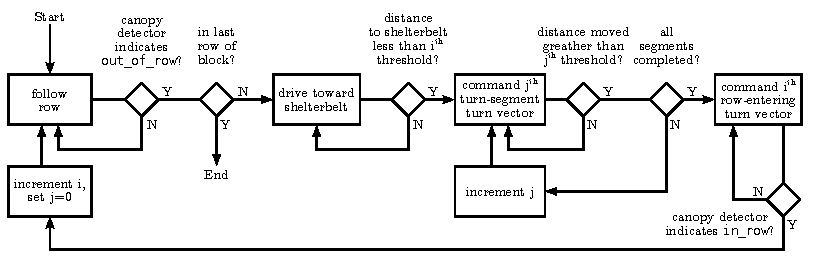
\includegraphics[width=\linewidth]{imgs/turning_diagrams/flowchart.pdf}
        \caption{
            Flow-chart of the developed autonomous block traversal algorithm.
        }
        \label{fig:turn_diagram}
    \end{figure}

    Figure~\ref{fig:turn_diagram} depicts the steps taken when traversing an orchard block.
    The multi-layer lidar is used to detect whether the vehicle is \textit{in\_row} or \textit{out\_of\_row} based on the presence of canopy above.
    A row-end turn sees the platform execute a series of turn segments which have previously been tuned for the specific row number and turn direction.
    Initially, a template set of turn-segments is executed at each row's end while under observation.
    If the vehicle gets too close to obstacles or nearby boundaries during execution, the operator would intervene before collision occurs.

    A complete row-end turn contains any number of segments.
    A `turn segment' is simply a vector and an end condition.
    Once the operator intervenes, he/she will tweak relevant parameters of the turn.
    This can be widening or tightening as well as lengthening or shortening the distance or angle of each segment.
    Finally, if an object is detected in the vehicle's path during a turn, the steering is automatically adjusted to avoid the object.
    This happens independently from the parameters contained in the map file.
    Figure~\ref{fig:suzy_turning} shows the platform performing a row-end turn while under autonomous control.

    \begin{figure}[htb]
        \centering
        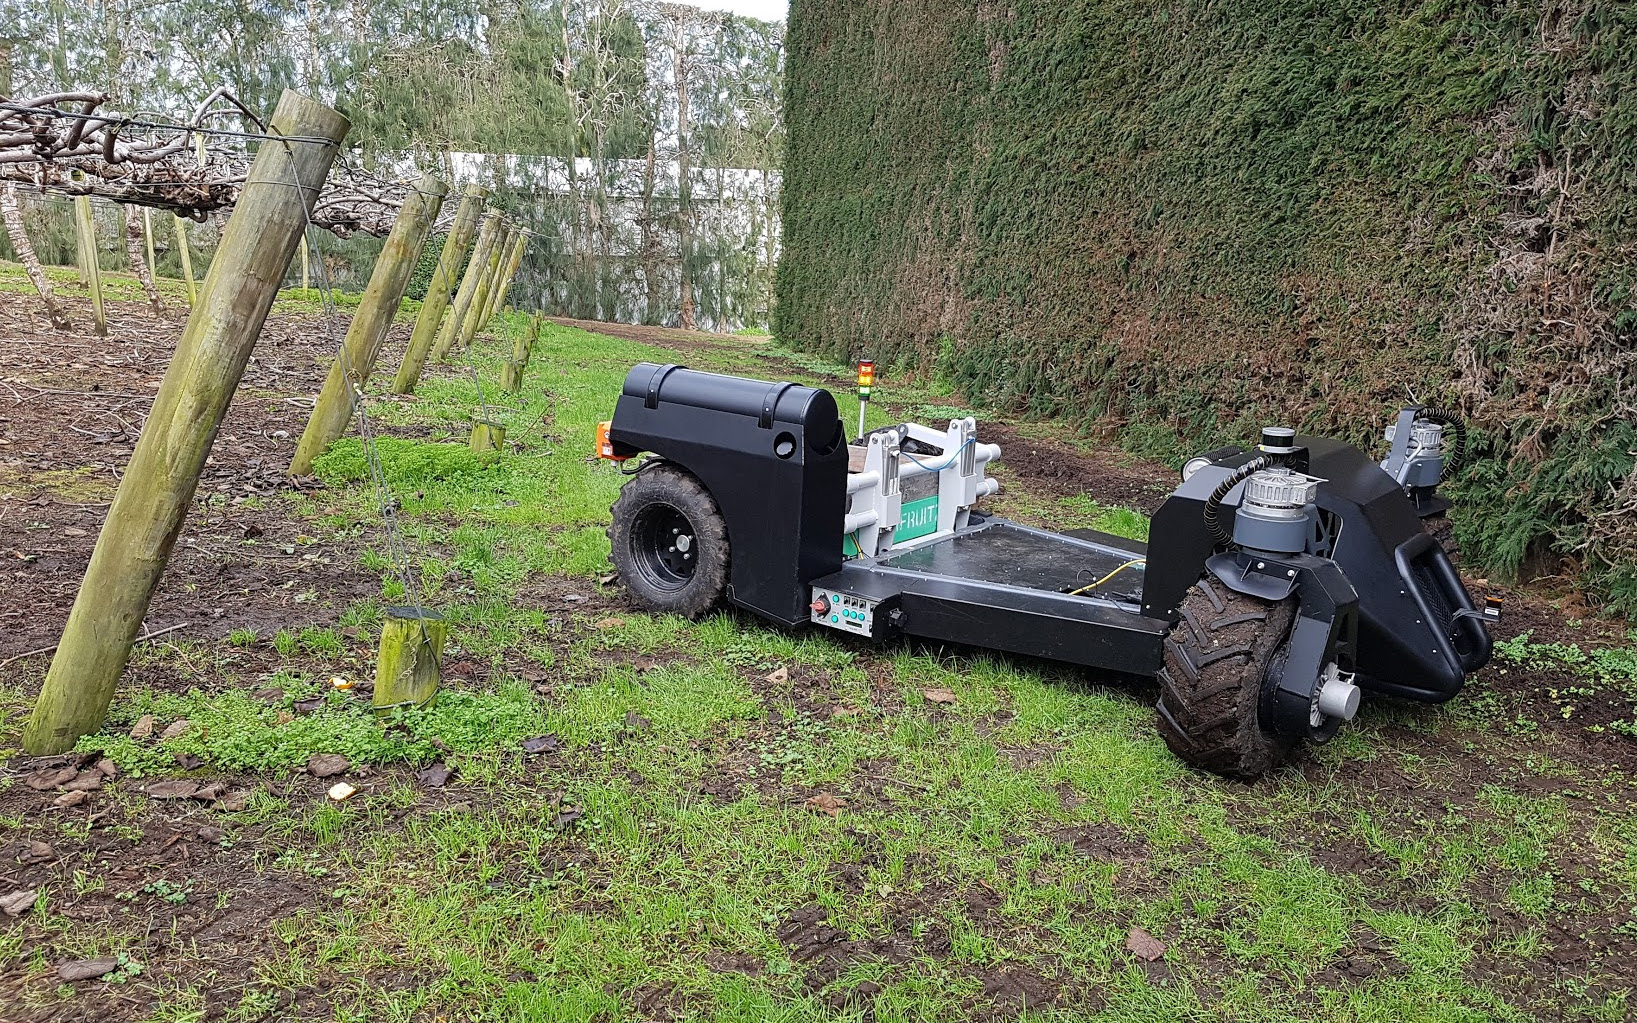
\includegraphics[width=\linewidth]{imgs/photos/suzy_turning.jpg}
        \caption{
            A row end turn being performed autonomously by the platform.
            The multi-layer lidar (Velodyne VLP-16) is visible above the front-right steering motor.
        }
        \label{fig:suzy_turning}
    \end{figure}

\section{Testing}
\label{sub:testing}

  \subsection{Mass Loading}
    Structural integrity testing was carried out by mounting a \SI{1100}{\kilo\gram} mass to the vehicle's module area.
    No deflection of the vehicle's chassis structure was evident upon application of the test mass.
    Deflection of \SI{1.5}{\milli\meter} was measured between the front pivot and the wheel supports.
    % \begin{figure}[htb]
    %     \centering
    %     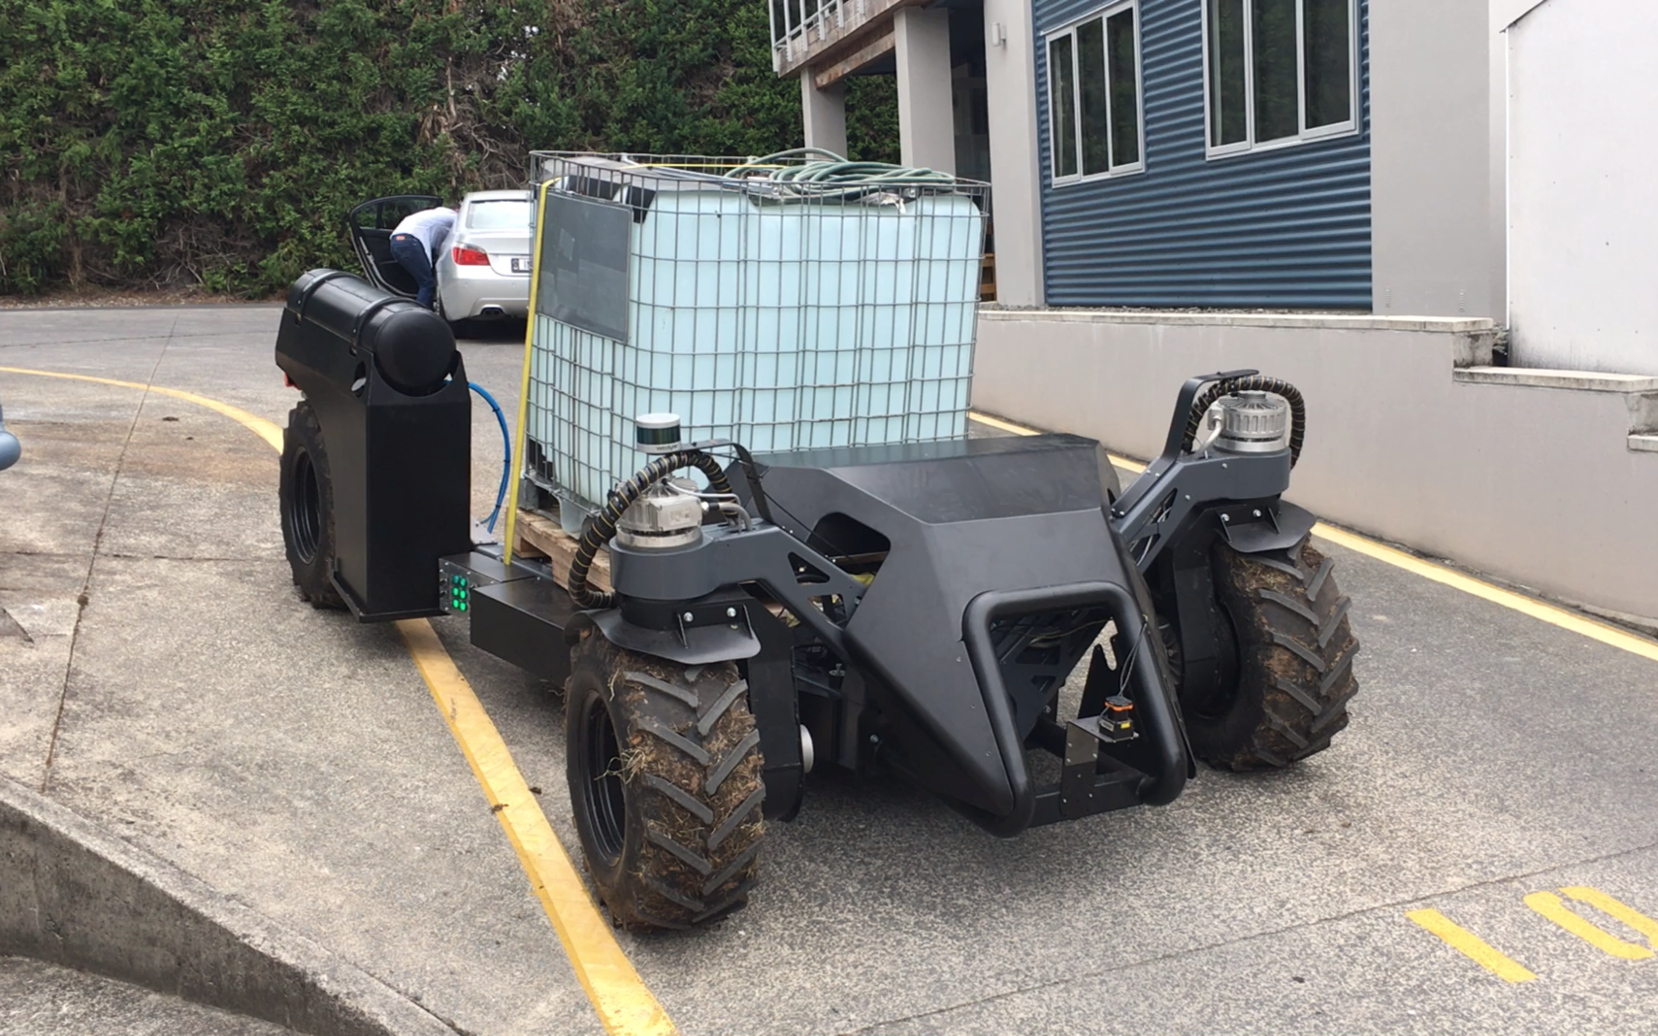
\includegraphics[width=\linewidth]{imgs/photos/stopTesting.jpg}
    %     % 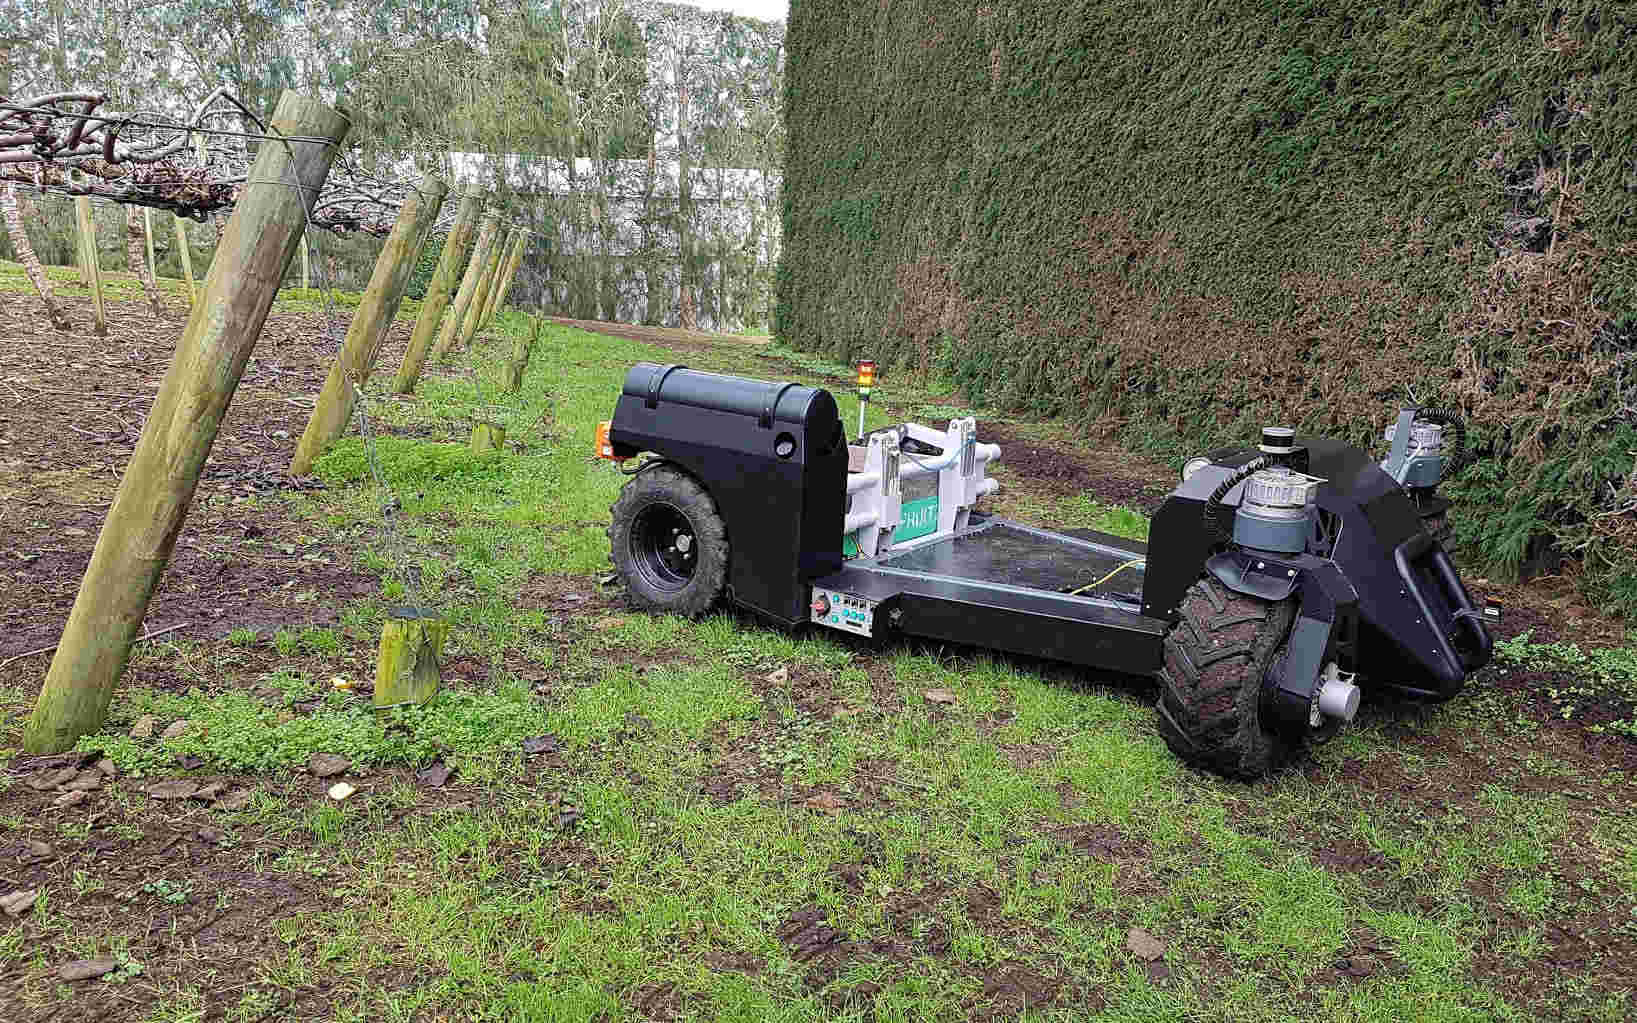
\includegraphics[width=\linewidth]{imgs/photos/suzy_turning_small.jpg}
    %     \caption{
    %         Stop testing down a \SI{10}{\degree} slope with a \SI{1100}{\kilo\gram} mass strapped to the module area.
    %     }
    %     \label{fig:suzy_testing}
    % \end{figure}
    Static steering tests conducted on a dry concrete surface showed no reduction in ability to turn while loaded with the test mass.
    Dynamic tests involved three instances of stopping at a \SI{10}{\degree} descent at a speed of \SI{10}{\kilo\meter\per\hour}.
    During each test the vehicle came to a complete stop within \SI{2.0}{\meter}.

  \subsection{Drive System}

    \begin{figure}[htb]
        \centering
        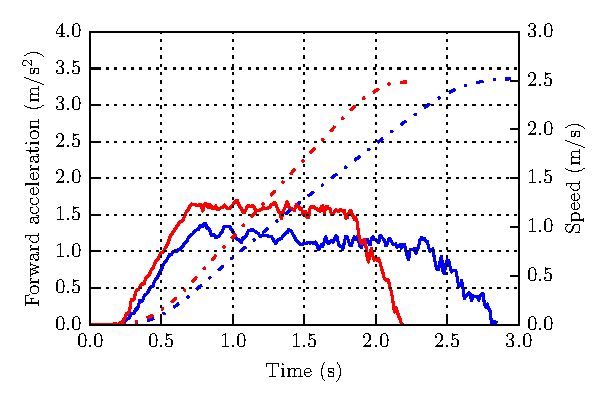
\includegraphics{imgs/drive_system/graph_acceleration.pdf}
        \caption{
            Acceleration of the platform on level ground (red) and up a \SI{3.5}{\degree} incline (blue).
        }
        \label{fig:acceleration}
    \end{figure}

    Drive system testing saw the platform accelerated from a stand-still under manual control to its maximum speed on both level ground and whilst climbing \SI{3.5}{\degree} incline.
    The acceleration was measured using an Inertial Measurement Unit (IMU, LPMS-USBAL2).
    Figure~\ref{fig:acceleration} shows the acceleration profile of the platform during both tests.
    The platform's weight during the test was estimated to have been \SI[separate-uncertainty=true]{850(50)}{\kilo\gram} in each case.

    In both instances the vehicle reached a top speed of \SI{2.5}{\meter\per\second} (\SI{9.0}{\kilo\meter\per\hour}), \SI{0.28}{\meter\per\second} short of the target speed.
    During the acceleration test on level ground, a peak power of between \SIrange{684}{770}{\watt}, and torque of between \SIrange{930}{1046}{\newton\meter} was calculated per wheel.
    During the inclined acceleration test, a peak power of between \SIrange{542}{610}{\watt}, and torque of between \SIrange{779}{876}{\newton\meter} was calculated per wheel.
    The torque calculations suggest the motors are developing their specified output of \SI{816}{\newton\meter}.
    The motor controllers are configured to supply extra torque for short bursts, which could explain why the calculated torque on level-ground is higher than this value.
    The inclined test began with the vehicle being held stationary using torque-control, which may have affected the controller's ability to produce the higher peak torque in this case.
    The lower than expected top speed in both cases suggest there are configuration issues with the motor controller's speed setting.

  \subsection{Turning Circle}

    Measurements of the vehicle's turning radius were performed at speeds of \SI{1.39}{\meter\per\second} (\SI{5.0}{\kilo\meter\per\hour}) and \SI{2.78}{\meter\per\second} (\SI{10.0}{\kilo\meter\per\hour}) on both dry tarmac and damp grassland.
    These speeds were calculated at the mid-point between the two front wheels.
    Having a wheelbase of \SI{2.67}{\meter}, these speeds equate to angular velocities of \SI{0.520}{\radian\per\second} and \SI{1.04}{\radian\per\second} respectively.

    In each test, a line was drawn on the ground in front of the vehicle to mark its starting position.
    The vehicle was then turned through an angle of \SI[separate-uncertainty=true]{180(10)}{\degree} under manual control with the steering angle set at \SI{90}{\degree}.
    The final angle was adjusted using odometry information to ensure the total angle was within \SI[separate-uncertainty=true]{180(3)}{\degree}.
    A marker was then drawn on the ground at the front of the vehicle at this position.
    The distance between the markers was measured at \SI{6.45}{\meter} for both surface types and both test speeds.
    This gives a turning radius of \SI{3.23}{\meter}, \SI{0.05}{\meter} wider than the estimate based on kinematic calculations.
    The authors put this discrepancy down to the accuracy of the angular calibration of the front wheels.

    % \begin{table}[htbp]
    %   \centering
    %   \footnotesize
    %   \begin{tabular}{ l | r r | r r | r r }

    %       \textbf{Test} & \multicolumn{2}{c}{\textbf{Tarmac}} & \multicolumn{2}{c}{\textbf{Gravel}} & \multicolumn{2}{c}{\textbf{Grass}}\\ \hline
    %                     & \SI{1.39}{\meter\per\second} & \SI{2.78}{\meter\per\second}     & \SI{1.39}{\meter\per\second} & \SI{2.78}{\meter\per\second}     & \SI{1.39}{\meter\per\second} & \SI{2.78}{\meter\per\second}   \\ \hline
    %       1 & 2.90 & 2.78 & 2.84 & 2.78 & 2.79 & 2.74\\
    %       2 & 2.90 & 2.78 & 2.84 & 2.78 & 2.79 & 2.74\\
    %       3 & 2.90 & 2.78 & 2.84 & 2.78 & 2.79 & 2.74\\
    %       4 & 2.90 & 2.78 & 2.84 & 2.78 & 2.79 & 2.74\\
    %       5 & 2.90 & 2.78 & 2.84 & 2.78 & 2.79 & 2.74\\
    %   \end{tabular}
    %   \caption{Results of turn-radius testing on three surface types and at two speeds.}
    %   \label{table:row_follow_path_lenghts}
    % \end{table}

    % Results from these tests are shown in \ref{table:row_follow_path_lenghts}.
    % They highlight issues with the turning capability of the vehicle.
    % Notice that the measured radius at the higher speed is less than that at lower speeds.
    % Also, variation is much lower at the higher speed (\SI{0.04}{\meter}) versus (\SI{0.11}{\meter}) at the slow speed.





    % TODO{Mark}: Re-read from here onwards
  \subsection{Bin Lifter}

    A pallet-mounted mass of \SI{370}{\kilo\gram} was used to test the bin lifter.
    The lifter's pneumatic valve block was manually activated until the pallet sat \SI{250}{\milli\meter} above the ground.
    To raise the load, pneumatic pressure of \SI{800}{\kilo\pascal} was applied to one port of each double acting cylinder while the other port was open to atmosphere.
    Lowering was done by opening both ports to atmosphere and allowing the load to descend under its own weight.
    This process was repeated five times.
    Additionally, the vehicle was driven \SI{300}{\meter} with the load, including an \SI{3.5}{\degree} incline for \SI{30}{\meter}.

    The lifting capacity of the mechanism was sufficient to raise the load gently to its target height.
    At its lower position, signs of imbalance between the two cylinders was evident that caused shuddering.
    This shuddering was caused by excessive and unbalanced static-friction between both sides of the four-bar mechanism, caused from over-tight sleeve bearings.
    The behaviour was also evident when hand actuating the lifter.
    Whilst driving, the load dropped by between \SIrange{60}{70}{\milli\meter} from its initial height.
    This drop, and the variation in resting position, was thought to be caused by the combination of static friction and driving related vibrations.

  \subsection{Turning Between Rows}

    Two orchard blocks (from different orchards) were used for row-turn testing.
    These blocks will be referred to as blocks A and B.
    Block~A was \SI{1.15}{\kilo\meter} in total traversable length spread over 10 rows, while block B was \SI{670}{\meter} in total traversable length spread over 9 rows.
    After tuning the row-end turning manoeuvres, our platform navigated block~A consecutively 7 times.
    Figure~\ref{fig:block_traversal_bateman} shows the number of interventions per traversal within block~A.
    A total of 19 traversals were used to tune the turns in this orchard.
    After tuning the row end-turns in block~B, it was navigated 3 times consecutively.
    Figure~\ref{fig:block_traversal_newnham} shows the number of interventions per traversal while under tuning in block~B, with 10 traversals in total.
    % This equates to a total of \SI{10}{\kilo\meter} of successfully navigated orchard rows.

    \begin{figure}[htb]
        \centering
        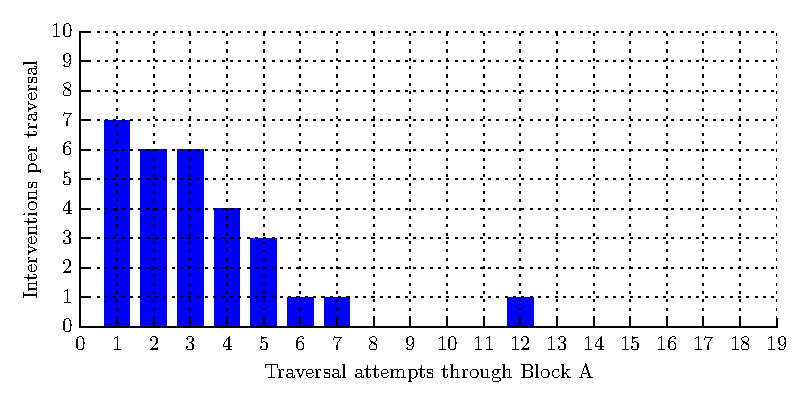
\includegraphics{imgs/tuning_graphs/bateman.pdf}
        \caption{
            Number of interventions during tuning of row-end turns throughout block A.
        }
        \label{fig:block_traversal_bateman}
    \end{figure}

    \begin{figure}[htb]
        \centering
        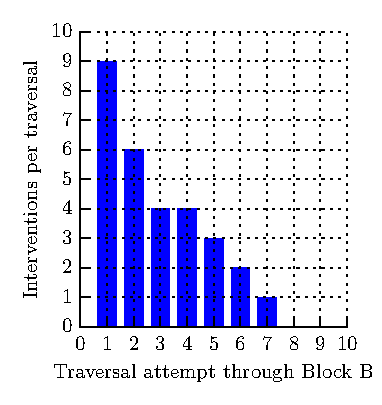
\includegraphics{imgs/tuning_graphs/newnham.pdf}
        \caption{
            Number of interventions during tuning of row-end turns throughout block B.
        }
        \label{fig:block_traversal_newnham}
    \end{figure}

    The key weakness of the current navigation system is the need to tune the row-end turns manually for each site.
    The tuning required for the first orchard block amounted to eight traversals of the entire block.
    For the second block, seven complete traversals were required for tuning.
    This creates a significant resource overhead for deployment to any new sites.
    If the turns are not sufficiently tuned, two types of failure occur.
    The most common case is that the vehicle turns between rows too tightly or not tightly enough and the object avoidance system is not sufficiently responsive to avoid a collision.
    All but four interventions were due to an imminent collision with a post during a row-end turn.
    Three interventions during row-end turning were due to the platform trying to recommence row following before facing the new target row.
    In this case the most feasible path for row following was detected along the headland area - instead of through the target row.
    One intervention, attempt 12 of block~A, was caused by the canopy detection system triggering a row-end turn whilst still inside a row.

  \subsection{Row Following}
    Row following repeatability tests were made by allowing the platform to self-drive through a row, from the same starting point, five times.
    The algorithm used was similar to that reported in \cite{Bell2016}, but had a couple of alterations.
    It used only a multi-layer lidar (Velodyne VLP-16) and an IMU (LPMS-USBAL2), but made no attempt to avoid obstacles.
    Its end-of-row detector was based on the vehicle's proximity to the row's last pair of posts, as opposed to detecting the absence of canopy above.

    Each test was conducted at the vehicle's target operating speed of \SI{1.39}{\meter\per\second} (\SI{5}{\kilo\meter\per\hour}).
    To determine the vehicle's trajectory, recordings of the lidar and IMU were made and post-processed using a SLAM package off-line.
    The SLAM package used was Cartographer (version 1.0) used as a ROS package.
    It produced both the map and the vehicle's trajectory information \citep{Hess2016}.
    The spacial resolution of the SLAM map was \SI{0.05}{\meter\per pixel}.
    Wheel odometry provided by the drive motors was not used during row following as signs of slippage were apparent.
    Quick measurements conducted on grass showed a velocity imbalance of approximately \SI{5}{\percent} between the rear wheels whilst driving forward.

    \begin{figure}[htb]
        \centering
        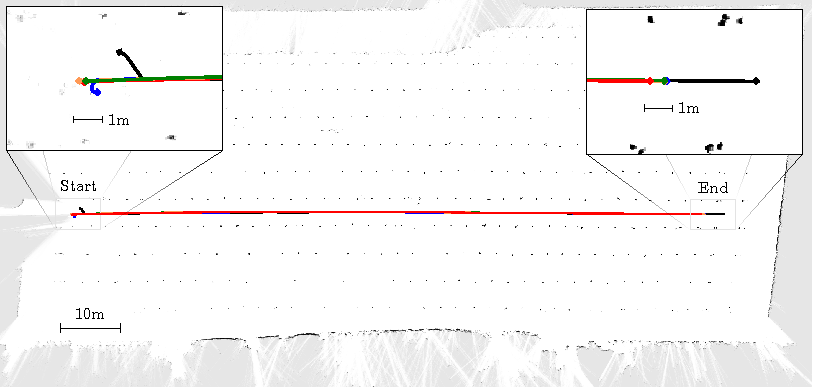
\includegraphics[width=\linewidth]{imgs/slam/paths2.pdf}
        \caption{
            Five trajectories recorded during five row-following repeatability tests.
        }
        \label{fig:row_following_paths}
    \end{figure}

    \begin{table}[htbp]
      \centering
      \footnotesize
      \begin{tabular}{ l l}

          \textbf{Test number}      &\textbf{Path length} \\ \hline
          1 & \SI{106.66}{\meter}\\
          2 & \SI{103.70}{\meter}\\
          3 & \SI{104.13}{\meter}\\
          4 & \SI{104.47}{\meter}\\
          5 & \SI{104.37}{\meter}\\
      \end{tabular}
      \caption{Total path length for each row-following test. The average length is \SI{104.67}{\meter} and the range is \SI{2.96}{\meter} (\SI{2.82}{\percent}).}
      \label{table:row_follow_path_lenghts}
    \end{table}

    \begin{figure}[htb]
        \centering
        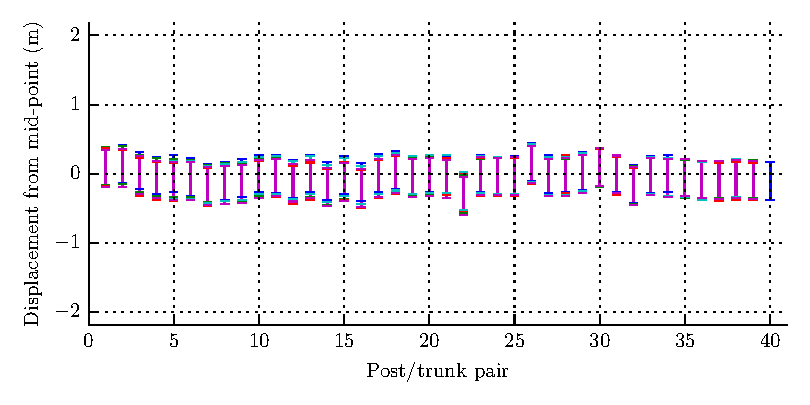
\includegraphics{imgs/slam/row_tracking_averages.pdf}
        \caption{
            Deviation between vehicle's tracking point and each post/trunk pair midpoint over five trials.
            The mean row width was \SI{4.35}{\meter}.
            % The y-axis is scaled to the mean row width (\SI{4.35}{\meter}).
            % The resolution of the generated SLAM map contributes $\pm$\SI{0.274}{\meter} of error.
        }
        \label{fig:row_following_performance_analysis}
    \end{figure}

    \begin{figure}[htb]
        \centering
        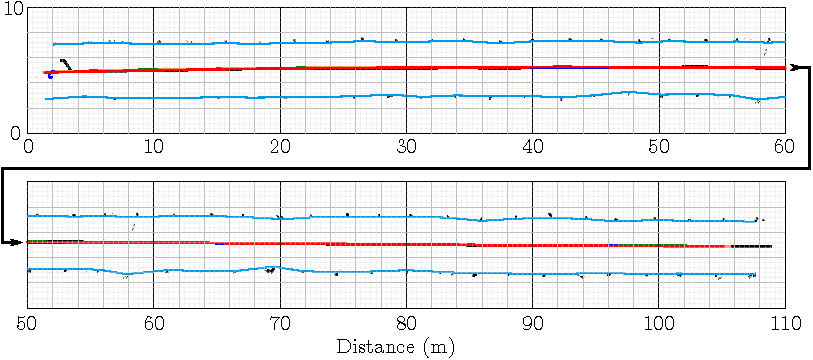
\includegraphics[width=\linewidth]{imgs/slam/row_tracking_segmented.pdf}
        \caption{
            Row-following paths shown relative to row boundaries.
            Boundary lines are linked with blue lines.
        }
        \label{fig:row_following_paths_segmented}
    \end{figure}

    \begin{figure}[htb]
        \centering
        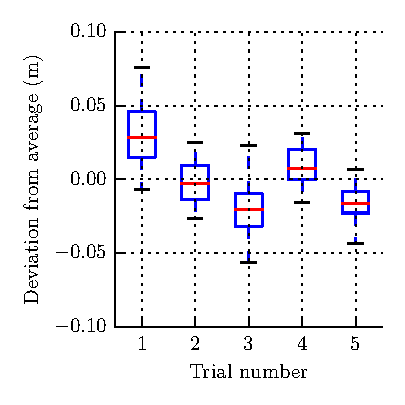
\includegraphics{imgs/slam/row_tracking_repeatability.pdf}
        \caption{
        Repeatability analysis of five row-following trials.
        Whiskers represent maximum deviations in both the positive and negative directions.
        Each trial has a sample size of 40.
        }
        \label{fig:row_following_repeatability}
    \end{figure}


    \begin{figure}[htb]
        \centering
        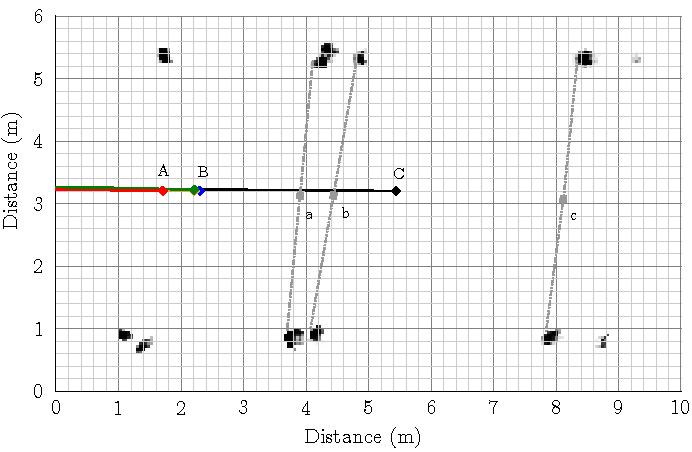
\includegraphics{imgs/slam/paths_end_points.pdf}
        \caption{
            Graph showing row-following end positions relative to tracked row features.
            Grey dotted lines connect row feature pairs, with squares indicating their mid-points.
        }
        \label{fig:row_following_end_points}
    \end{figure}

    Figure~\ref{fig:row_following_paths} shows the resulting orchard map and five trajectories overlaid on top of each other.
    While differences in start position are estimated to be less than \SI{0.1}{\meter}, the trajectories show a spread of \SI{1.69}{\meter}.
    The total path length for each run is listed in Table \ref{table:row_follow_path_lenghts}.
    Figure~\ref{fig:row_following_performance_analysis} shows an analysis of the path following performance.
    This involved measuring the midpoints between each post/trunk pair manually using vector drawing software and comparing these midpoints to each path.
    Sources of error were $\pm$\SI{1} pixel at either end of the midpoint measurement lines as well as rounding errors.
    Figure~\ref{fig:row_following_repeatability} quantifies the divergence of each path from the average location recorded between each trunk/post pair.
    Figure~\ref{fig:row_following_end_points} shows the end-points for each run relative to the row features at the end of the row.

    Analysis of the tracking performance is particularly difficult as the positioning of the posts/trunks show obvious signs of deviation, evident in Figure~\ref{fig:row_following_paths_segmented}.
    For example, the dip at post/trunk pair twenty-two in Figure~\ref{fig:row_following_performance_analysis} corresponds with the post/trunk pair near the \SI{58}{\meter} mark in Figure~\ref{fig:row_following_paths_segmented}.
    Similarly, the peak at position 26 corresponds to the post/trunk pair near the \SI{70}{\meter} mark.
    Without significant corrections to the data, which would be subjective, the analysis describes more about the linearity of the orchard than the trajectory.
    It is apparent however from Figure~\ref{fig:row_following_paths_segmented} that the vehicle's path is relatively straight and remains unperturbed by the non-linearity in positioning of the row's features.

    Figure~\ref{fig:row_following_repeatability} quantifies the deviation between each trial relative to the mean path taken over the five trials.
    It shows that the worst case repeatability was less than $\pm$\SI{75}{\milli\meter}.

    Finally, Figure~\ref{fig:row_following_end_points} shows the end position of each path.
    The path-following algorithm determines the end position based on its proximity to the last post-pair within its detection range.
    Notice that the last post in each row is spaced slightly further than is usual inside the row.
    This is visible along the left hand side of the SLAM map shown in Figure~\ref{fig:row_following_paths}.
    That extra spacing places the final post-pair near the software-defined cut-off region used to identify post/trunk pairs.
    Stopping slightly earlier results in the last post/trunk pair not being detected, as is the case in path groups A and B.
    Additionally, there is ambiguity in the position of the second-to-last post/trunk pair because vines have been planted in close proximity to the posts.
    Analysis of the recorded sensor data shows this to be the cause of the separation in end-positions between points A and B.

\section{Discussion}
\label{sect:discussion}

    The reported platform meets the specified requirements and has proved its usefulness during three pollination and harvesting seasons.
    However, during these operations the vehicle was mostly operated under manual control because of the need to drive close to row boundaries.
    The width of the vehicle and modules meant it was necessary to perform two passes through each row in order to access the full canopy area.
    The vehicle's overall height is \SI{1.25}{\meter}, leaving \SI{0.15}{\meter} between it and the target ceiling height of \SI{1.4}{\meter}.

    Results from navigation tests indicate that multi-layer lidar with wheel-encoder feedback is sufficient for row turning tasks.
    For row following, an IMU and multi-layer lidar based algorithm produced paths that were sufficiently repeatable and close to the row's centre-line.
    Wheel slippage meant encoder information was less suitable for long-term odometry than the odometry information provided by the SLAM package, which was based on processed lidar and IMU data.
    While more accurate for longer-term path tracking, the short-term response is not as accurate as encoder or IMU based odometry.
    Future work will combine all three sources into a single output with improved short and long-term accuracy.

    The method for turning between rows calls for further work.
    Row end turning was a manual process that involved observing an autonomously driven turn and manually adjusting the length or radius of path segments.
    Future work will focus on enabling the system to plan row-end turns based on perception based sensor data -- without a manually created map.
    Observationally, detecting row end-points based on the vehicle's proximity to the last post-pair proved more reliable than detecting the presence/absence of canopy.

    The platform's \SI{96}{\volt} battery pack and electrical system introduced a electrical hazard during development.
    % While essential for safety, risk mitigation procedures added complexities and delays that could have been avoided by simply selecting a lower operating voltage.
    The authors suggest a voltage of \SI{48}{\volt} as it bears a reduced risk of injury from shock.
    Inputs of \SI{48}{\volt} are supported across a wider range of motors, motor controllers, and power converters, but cabling requirements are increased.

    The series-hybrid electrical configuration allowed the vehicle to drive and provide power to subsystems without running the petrol engine.
    This was useful in testing scenarios, where people are in close proximity to the vehicle, as it eliminated exhaust fumes and reduced noise and vibration.
    However, robotic modules and the bin-lifting mechanism required pneumatic pressure to function.
    As the air-compressor was belt driven from the petrol engine it was necessary to frequently run the engine.
    An electric air-compressor would allow the system to run without the petrol engine for much longer periods.

    The use of more general purpose platforms to test navigation algorithms enabled the navigation software to be developed in parallel with the physical hardware.
    Their smaller size eliminated the risk of serious injury and led to a speed up in development and test cycles.
    It also meant that navigation testing could continue while the full-size platform was engaged in other activities.

    % Simulation of the robot hardware proved useful for finding software issues before implementation on hardware.
    % Much of the time developing the simulation went into the creation of a geometric model of the platform.
    % The model also proved useful for visualising the state of the vehicle and sensor outputs, using Rviz, in real-time and when replaying recorded sensor data.

\section{Conclusion}
    This work presents a platform designed specifically for autonomously transporting task-specific modules through pergola-style kiwifruit orchards.
    The platform is capable of carrying over twice the mass of similar platforms reported previously.
    The four wheel drive system with two individually-actuated steering wheels was well suited for use in and around kiwifruit orchards.
    The authors deem the use of a four-wheel steering configuration in this environment to be unnecessary.

    Various navigation sensors were trialled in the kiwifruit orchard environment.
    Multi-layer lidar proved to be the most versatile sensor for orchard based navigation owing to its wide field-of-view and robust outputs.
    Using a map of manually adjusted row-end turns, the platform has navigated over \SI{10}{\kilo\meter} of orchard rows using only wheel-encoders and a single multi-layer lidar.
    A significant amount of work was required to tune the row-end-turns, which has implications for commercial deployment.
    Row following tests using an algorithm based only on multi-layer lidar and IMU inputs proved to be repeatable to within $\pm$\SI{75}{\milli\meter}.

    % The authors recommend a system voltage of \SI{48}{\volt} for development platforms due to safety and component availability, which this platform did not use.
    The use of smaller, commercially available, robots proved valuable when developing navigation software due to their safety and portability.
    Future work will focus on developing the navigation system so that the vehicle can plan row-end turns and avoid obstacles whilst row following.


\section*{Acknowledgements}
This research was supported by the New Zealand Ministry for Business, Innovation and Employment (MBIE) on contract UOAX1414.
The authors acknowledge contributions from Phillip Ross, Gordon Neshausen, Josh Barnett, and Erin Simms who were involved with design and fabrication.

\bibliographystyle{model5-names}
\bibliography{bibliography_jamie,bibliography_mark}

\end{document}
